%Latex Template provided by Ivan Avramidi
%==========================================================
% DO NOT MODIFY THIS FILE <================================
%==========================================================
%
% This is a LATEX template for the Homework in MATH 352
% Just add your name in the space provided
% and type your solutions to each problem in the space below
%
%==========================================================
% DO NOT CHANGE ANYTHING ELSE <============================
%==========================================================
\documentclass[12pt]{article}
\usepackage{graphicx}
%========================
\def\cdate{{Fall 2021}}
%========================
\usepackage{amsmath,amsfonts,amssymb,txfonts}
\usepackage[table,xcdraw]{xcolor}
\textwidth=17truecm
\textheight=20truecm
\oddsidemargin=0pt
\evensidemargin=0pt
\parindent=0pt
\makeatother
\pagestyle{myheadings}
\markboth{\small\it
Semester Project  CSE 321: Internet and Web Programming. \cdate}
{\small\it 
Semester Project CSE 321: Internet and Web Programming. \cdate}
\makeatletter
\renewcommand{\@evenhead}{\raisebox{0pt}[\headheight][0pt]{\vbox{\hbox
to \textwidth{\thepage\hfil\strut\leftmark}\hrule}}}
\renewcommand{\@oddhead}{\raisebox{0pt}[\headheight][0pt]{\vbox{\hbox
to \textwidth{\rightmark\hfil\strut\thepage}\hrule}}}
\makeatother
%=========================================================
\begin{document}
\begin{titlepage}
%\thispagestyle{empty}
\null
\vspace{-40mm}
\hspace*{90truemm}{\hrulefill}\par\vskip-4truemm\par
\hspace*{90truemm}{\hrulefill}\par\vskip5mm\par
\hspace*{90truemm}{{\large\sc New Mexico Tech {\rm (\cdate)}}}\vskip4mm\par
\hspace*{90truemm}{\hrulefill}\par\vskip-4truemm\par
\hspace*{90truemm}{\hrulefill}
\par
\bigskip
\bigskip
\par
\vspace{3cm}
\centerline{\huge\bf Semester Project CSE 321:}
\bigskip
\centerline{\huge\bf Internet \& Web Programming}
\bigskip
\bigskip
\centerline{\Large\bf 
%================================================================
% INSERT YOUR NAME ON THE LINE BELOW <=====================
%================================================================
Orion Nassaux,
Alan Fenton,
Alexander Bair
}
\bigskip
\centerline{\it New Mexico Institute of Mining and Technology}
\centerline{\it Socorro, NM 87801, USA}

\bigskip
\centerline{Date: 
%================================================================
% INSERT THE DATE ON THE LINE BELOW <============================
%================================================================
\today
}
\vfill
\end{titlepage}
%=============================================================
This project is based around providing financial statistical analysis, because most banking websites are difficult to use, and don’t give you the tools to do a post-observation of your budget.

\par

    
    
    

%==================================================================
\par
%==================================================================
\section{Five Websites That are Relevant to the Theme:}
\subsection{PocketGuard}
Pocket Guard has the following features:
\begin{itemize}
    \item List savings, checking and credit accounts
    \item Offers free in-app savings account
    \item percentage of spending breakdown by month as 
    \item Spending by month as a line, compare months
    \item create own hashtags for analysis
    \item spending percentages by merchant by month
    \item automatically finds regular bills and pays checks
    \item sent budget goals category, and total
    \item shows net cash after budget goals
    \item saving goals (ie save for purchase)
    \item calculates net worth
    \item displays transaction
    \item displays opportunity for savings, (ie better phone plan)
\end{itemize}
    
\subsection{Mint}
\begin{itemize}
    \item Automatic transaction tagging
    \item Budgeting
    \item Set spending goals
    \item Aggregation of multiple accounts
    \item Net worth tracking
    \item Advanced Analytics
    \begin{itemize}
        \item Monthly Income to spending ratio
        \item Spending Habits
    \end{itemize}
\end{itemize}
\subsection{You Need a Budget (YNAB)}
You Need a Budget (YNAB) has the following features:
\begin{itemize}
    \item Focuses on living off of last months paycheck.
    \item set budgets
    \item create own hashtags for analysis
    \item shows net cash after budget goals
    \item Larger categories with smaller subdivisions
\end{itemize}

\subsection{EveryDollar}
\begin{itemize}
    \item Budgeting
    \item Debt Tracking
    \item Premium membership allows users to automatically tack transactions from their bank
    \item Percentage Breakdown of Budget (not actual amount spent)
    \item Requires an every dollar budget
\end{itemize}

\subsection{Goodbudget}
\begin{itemize}
    \item Budgeting
    \item Debt Tracking
    \item Manually add Transactions (Not automatic)
    \item Shows Advanced Analytics
    \begin{itemize}
        \item Percentage Breakdown of Amount Spent
        \item Spending vs Budget
        \item Income vs Spending
    \end{itemize}
\end{itemize}
\section{Functionality descriptions}
\subsection{Tagging}
The ability to mark certain transactions as belonging to one or more categories.
\subsection{Budgeting}
The ability to set a limit to the amount of money to be spent in a category.
\subsection{Percentage Breakdown}
The ability to review spending and determine what percent of spending was spent in a particular category.
\subsection{Spending Habits}
The ability to track previous purchases to provide heuristical data about spending. (You've spent 10\$ on coffee this month, less than your average of 15\$)
\subsection{Automatic Tracking}
The ability to add new transactions to the account without user input.
\subsection{Account Aggregation}
The ability to access multiple accounts and view combined analytics.

\pagebreak

\subsection{Our Website VS Existing Websites:}



\begin{table}[!h]
\begin{tabular}{|
>{\columncolor[HTML]{FFFFFF}}l |
>{\columncolor[HTML]{FFFFFF}}c |
>{\columncolor[HTML]{FFFFFF}}c |
>{\columncolor[HTML]{FFFFFF}}c |
>{\columncolor[HTML]{FFFFFF}}c |
>{\columncolor[HTML]{FFFFFF}}c |
>{\columncolor[HTML]{FFFFFF}}c |}
\hline
{\color[HTML]{333333} }           & \multicolumn{1}{l|}{\cellcolor[HTML]{FFFFFF}{\color[HTML]{333333} FinTool}} & \multicolumn{1}{l|}{\cellcolor[HTML]{FFFFFF}{\color[HTML]{333333} Mint}} & \multicolumn{1}{l|}{\cellcolor[HTML]{FFFFFF}{\color[HTML]{333333} PocketGuard}} & \multicolumn{1}{l|}{\cellcolor[HTML]{FFFFFF}{\color[HTML]{333333} YNAB}} & \multicolumn{1}{l|}{\cellcolor[HTML]{FFFFFF}{\color[HTML]{333333} EveryDollar}} & \multicolumn{1}{l|}{\cellcolor[HTML]{FFFFFF}{\color[HTML]{333333} Goodbudget}} \\ \hline
{\color[HTML]{333333} Tagging}                                                       &
{\color[HTML]{333333} V}                                                               & 
{\color[HTML]{333333} O}                                                              & 
{\color[HTML]{333333} V}                                                              & 
{\color[HTML]{333333} O}                                                              & 
{\color[HTML]{333333} V}                                                              & 
{\color[HTML]{333333} V}                                                              \\ \hline
{\color[HTML]{333333} Budgeting}                                                         &
{\color[HTML]{333333} V}                                                               & 
{\color[HTML]{333333} O}                                                              & 
{\color[HTML]{333333} V}                                                               & 
{\color[HTML]{333333} V}                                                              & 
{\color[HTML]{333333} V}                                                               & 
{\color[HTML]{333333} V}                                                               \\ \hline
{\color[HTML]{333333} Percentage Breakdown}                                             &
{\color[HTML]{333333} V}                                                               & 
{\color[HTML]{333333} V}                                                              & 
{\color[HTML]{333333} X}                                                              & 
{\color[HTML]{333333} X}                                                               & 
{\color[HTML]{333333} V}                                                              & 
{\color[HTML]{333333} V}                                                               \\ \hline
{\color[HTML]{333333} Spending Habits}                                                  &
{\color[HTML]{333333} V}                                                                & 
{\color[HTML]{333333} V}                                                               & 
{\color[HTML]{333333} X}                                                              & 
{\color[HTML]{333333} X}                                                               & 
{\color[HTML]{333333} V}                                                               & 
{\color[HTML]{333333} V}                                                              \\ \hline
{\color[HTML]{333333} Automatic Tracking}                                                  &
{\color[HTML]{333333} X}                                                                & 
{\color[HTML]{333333} V}                                                               & 
{\color[HTML]{333333} V}                                                              & 
{\color[HTML]{333333} V}                                                               & 
{\color[HTML]{333333} V}                                                               & 
{\color[HTML]{333333} X}                                                              \\ \hline
{\color[HTML]{333333} Account Aggregation}                                                  &
{\color[HTML]{333333} V}                                                                & 
{\color[HTML]{333333} V}                                                               & 
{\color[HTML]{333333} V}                                                              & 
{\color[HTML]{333333} V}                                                               & 
{\color[HTML]{333333} X}                                                               & 
{\color[HTML]{333333} V}                                                              \\ \hline
\end{tabular}
\end{table}

\section{Storyboard:}
\subsection{Target Audience:}
Our typical customers can be divided into two groups, personal users, and business users. In order to better shape the user stories, we are going to make some broad generalizations about these groups. Additionally, certain tags will automatically be generated or applied differently.\\
\subsubsection{Personal Users}
Personal users, for the most part have one or two credit/debit accounts, and usually only have to deal with their own expenses.\\
\subsubsection{Business Users}
By contrast, business users tend to have several credit/debit accounts, 3 or more, and are likely to want to make use of the more complex features, such as account aggregation.\\
\subsection{Design Prototype:}
\subsubsection{First Time Setup}
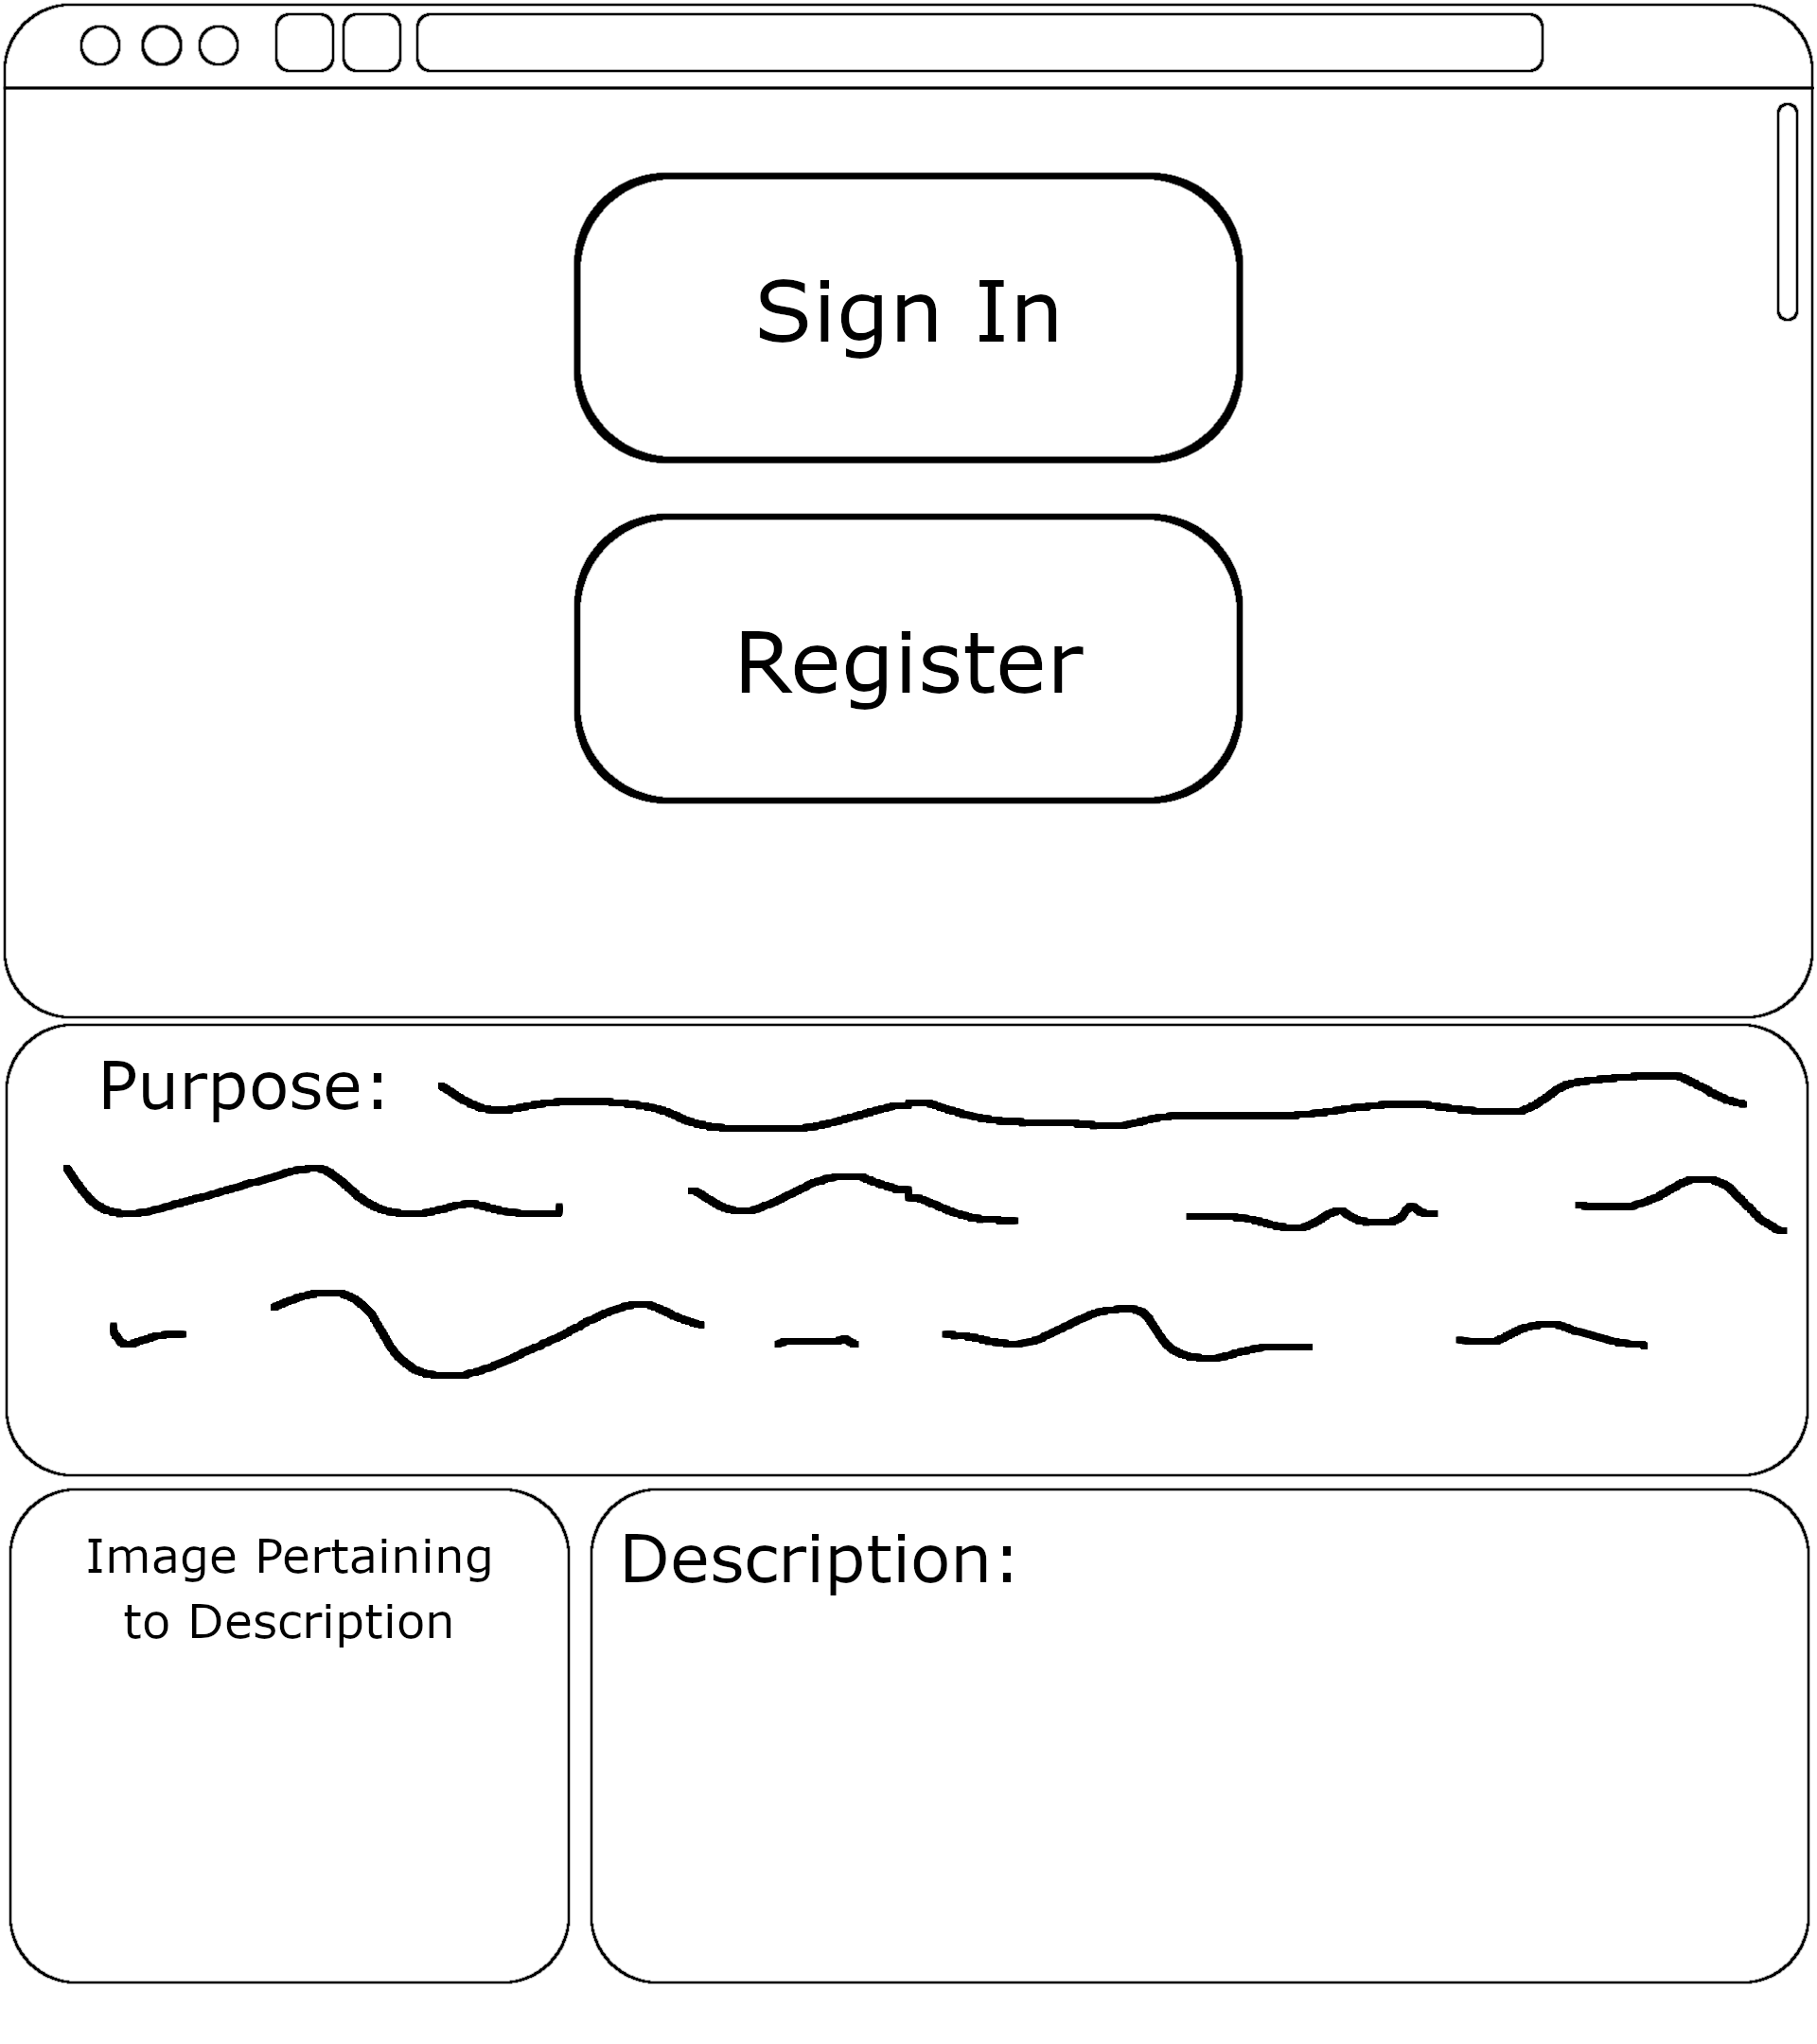
\includegraphics[width=3in]{HomePage.png}\\
This is the page users will land on when thy search for our site. If you already have an account you simply need to sign in, if you don't you need to register.\\

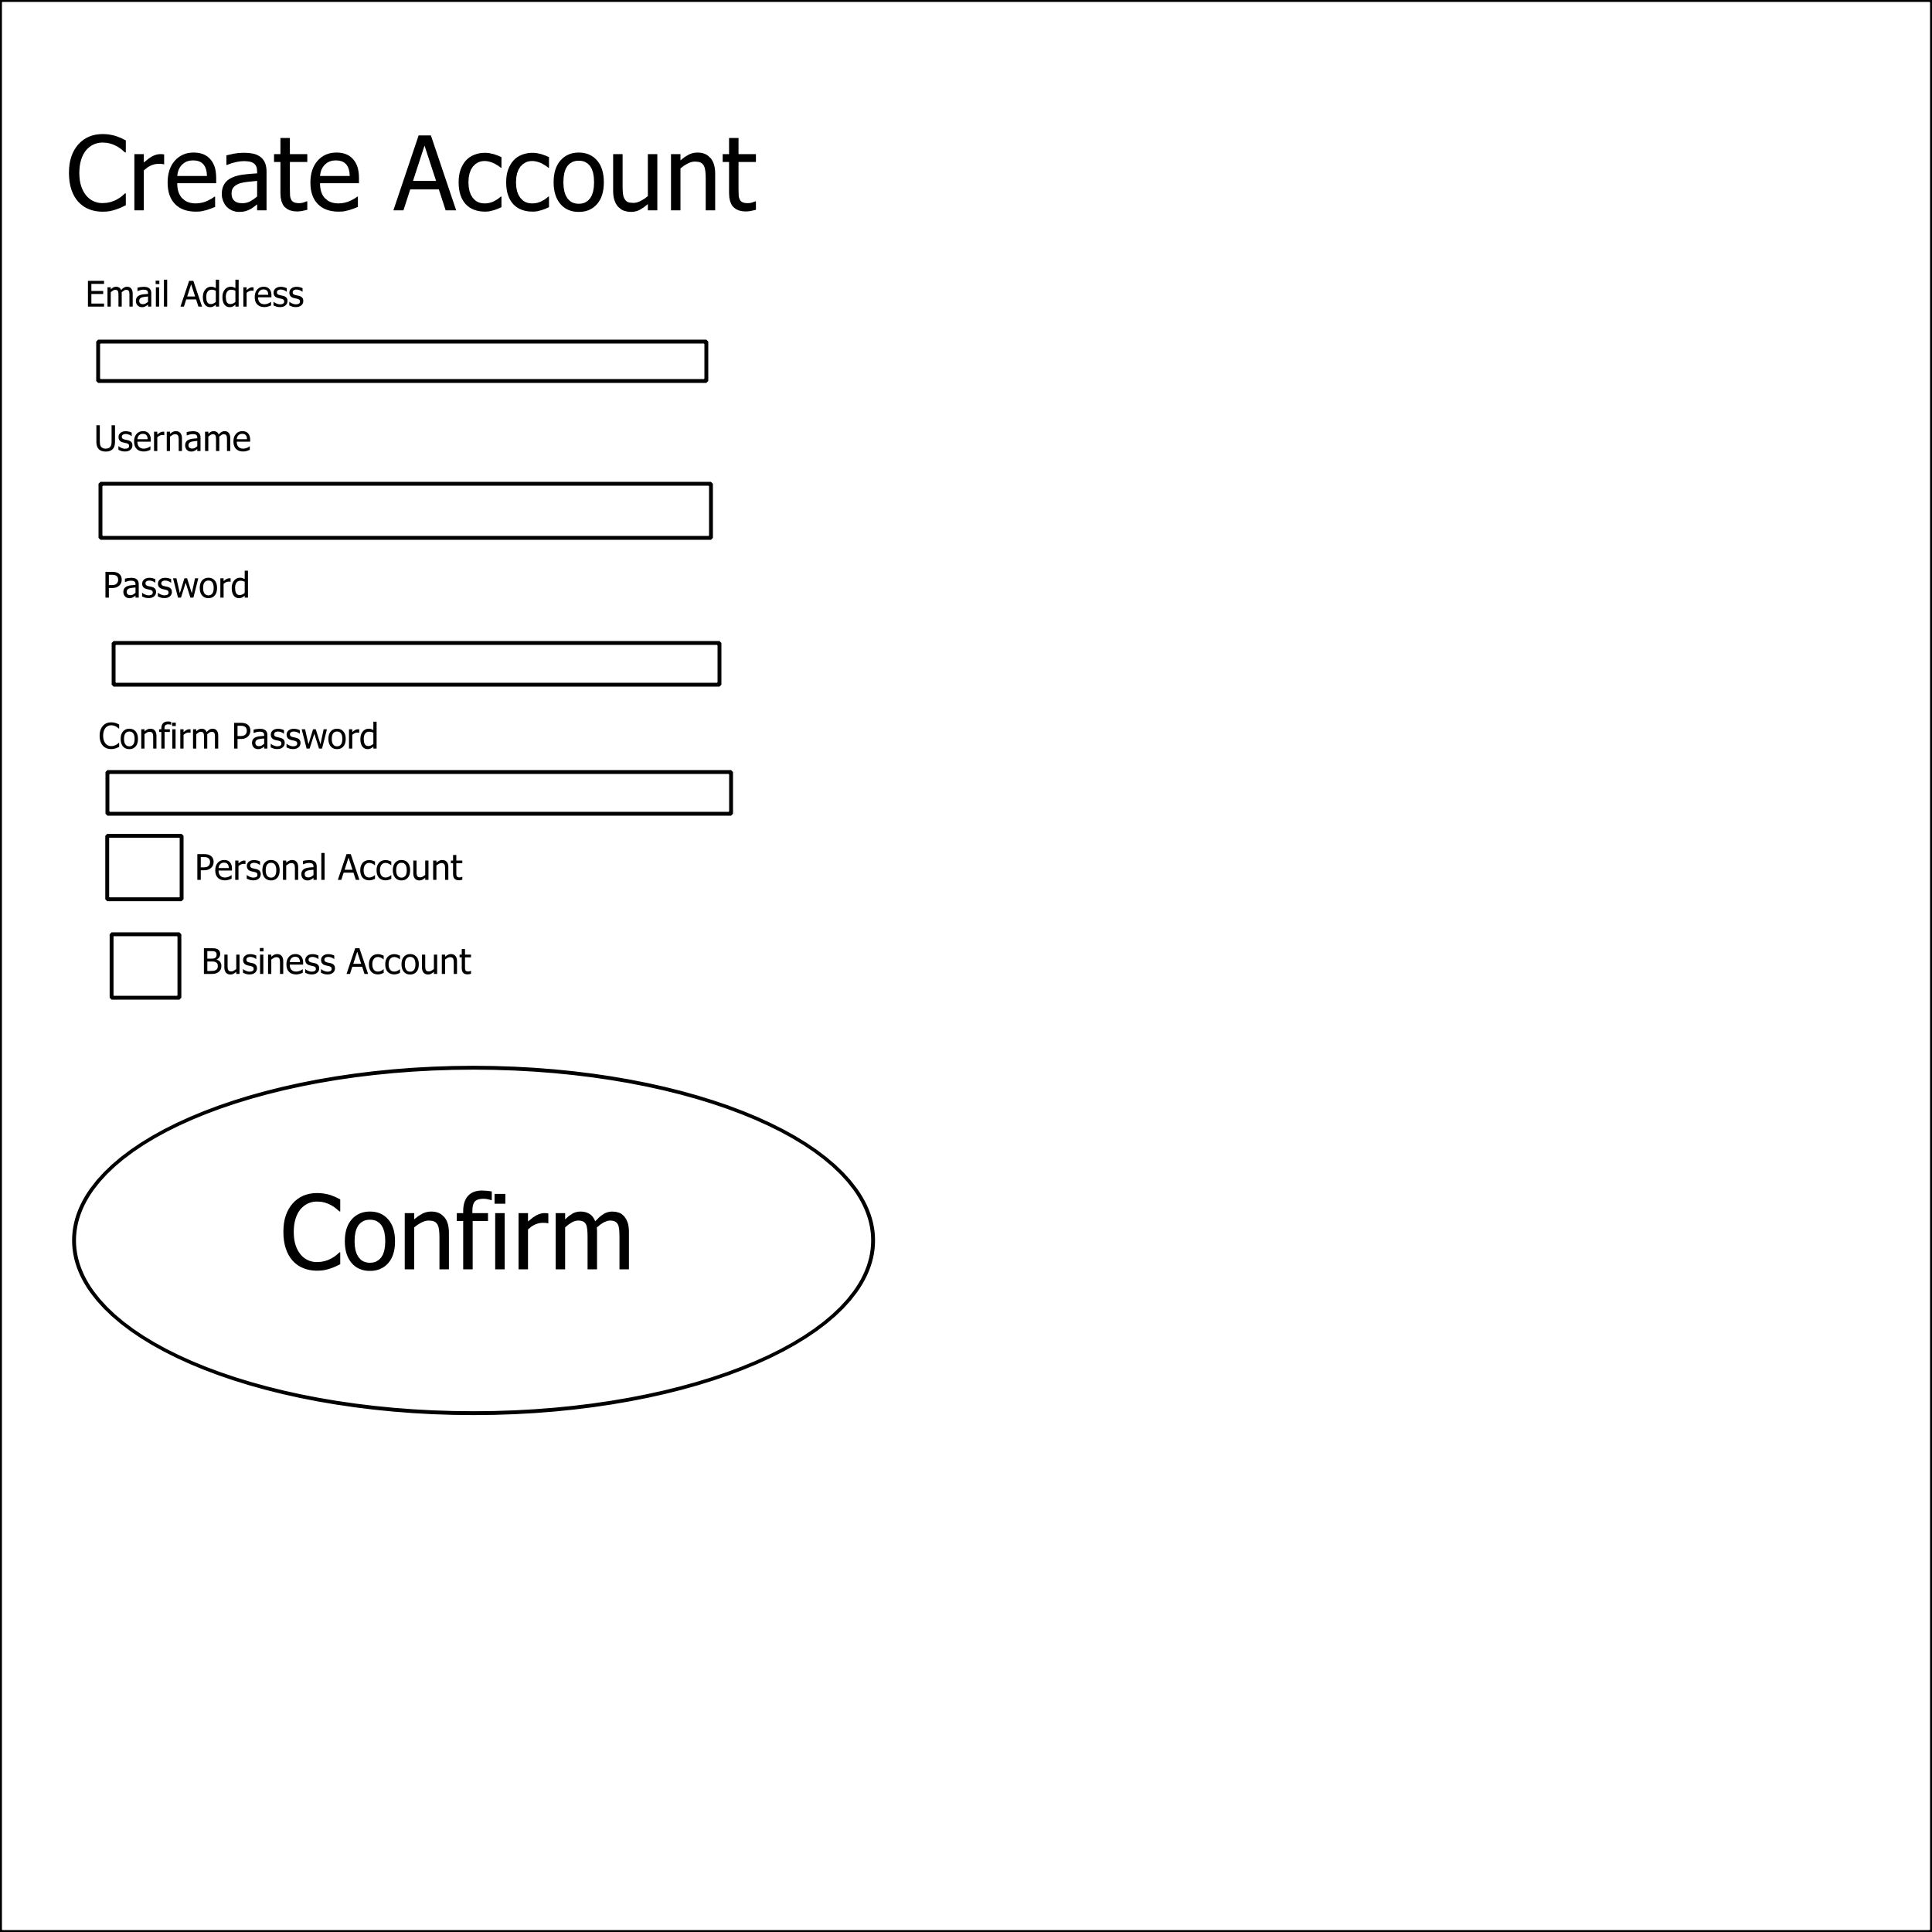
\includegraphics[width=3in]{create_account.jpg}\\
New users add their email address to create an account, choose whether is a personal or business account. This changes the default budgets and tags when the account is first created.\\

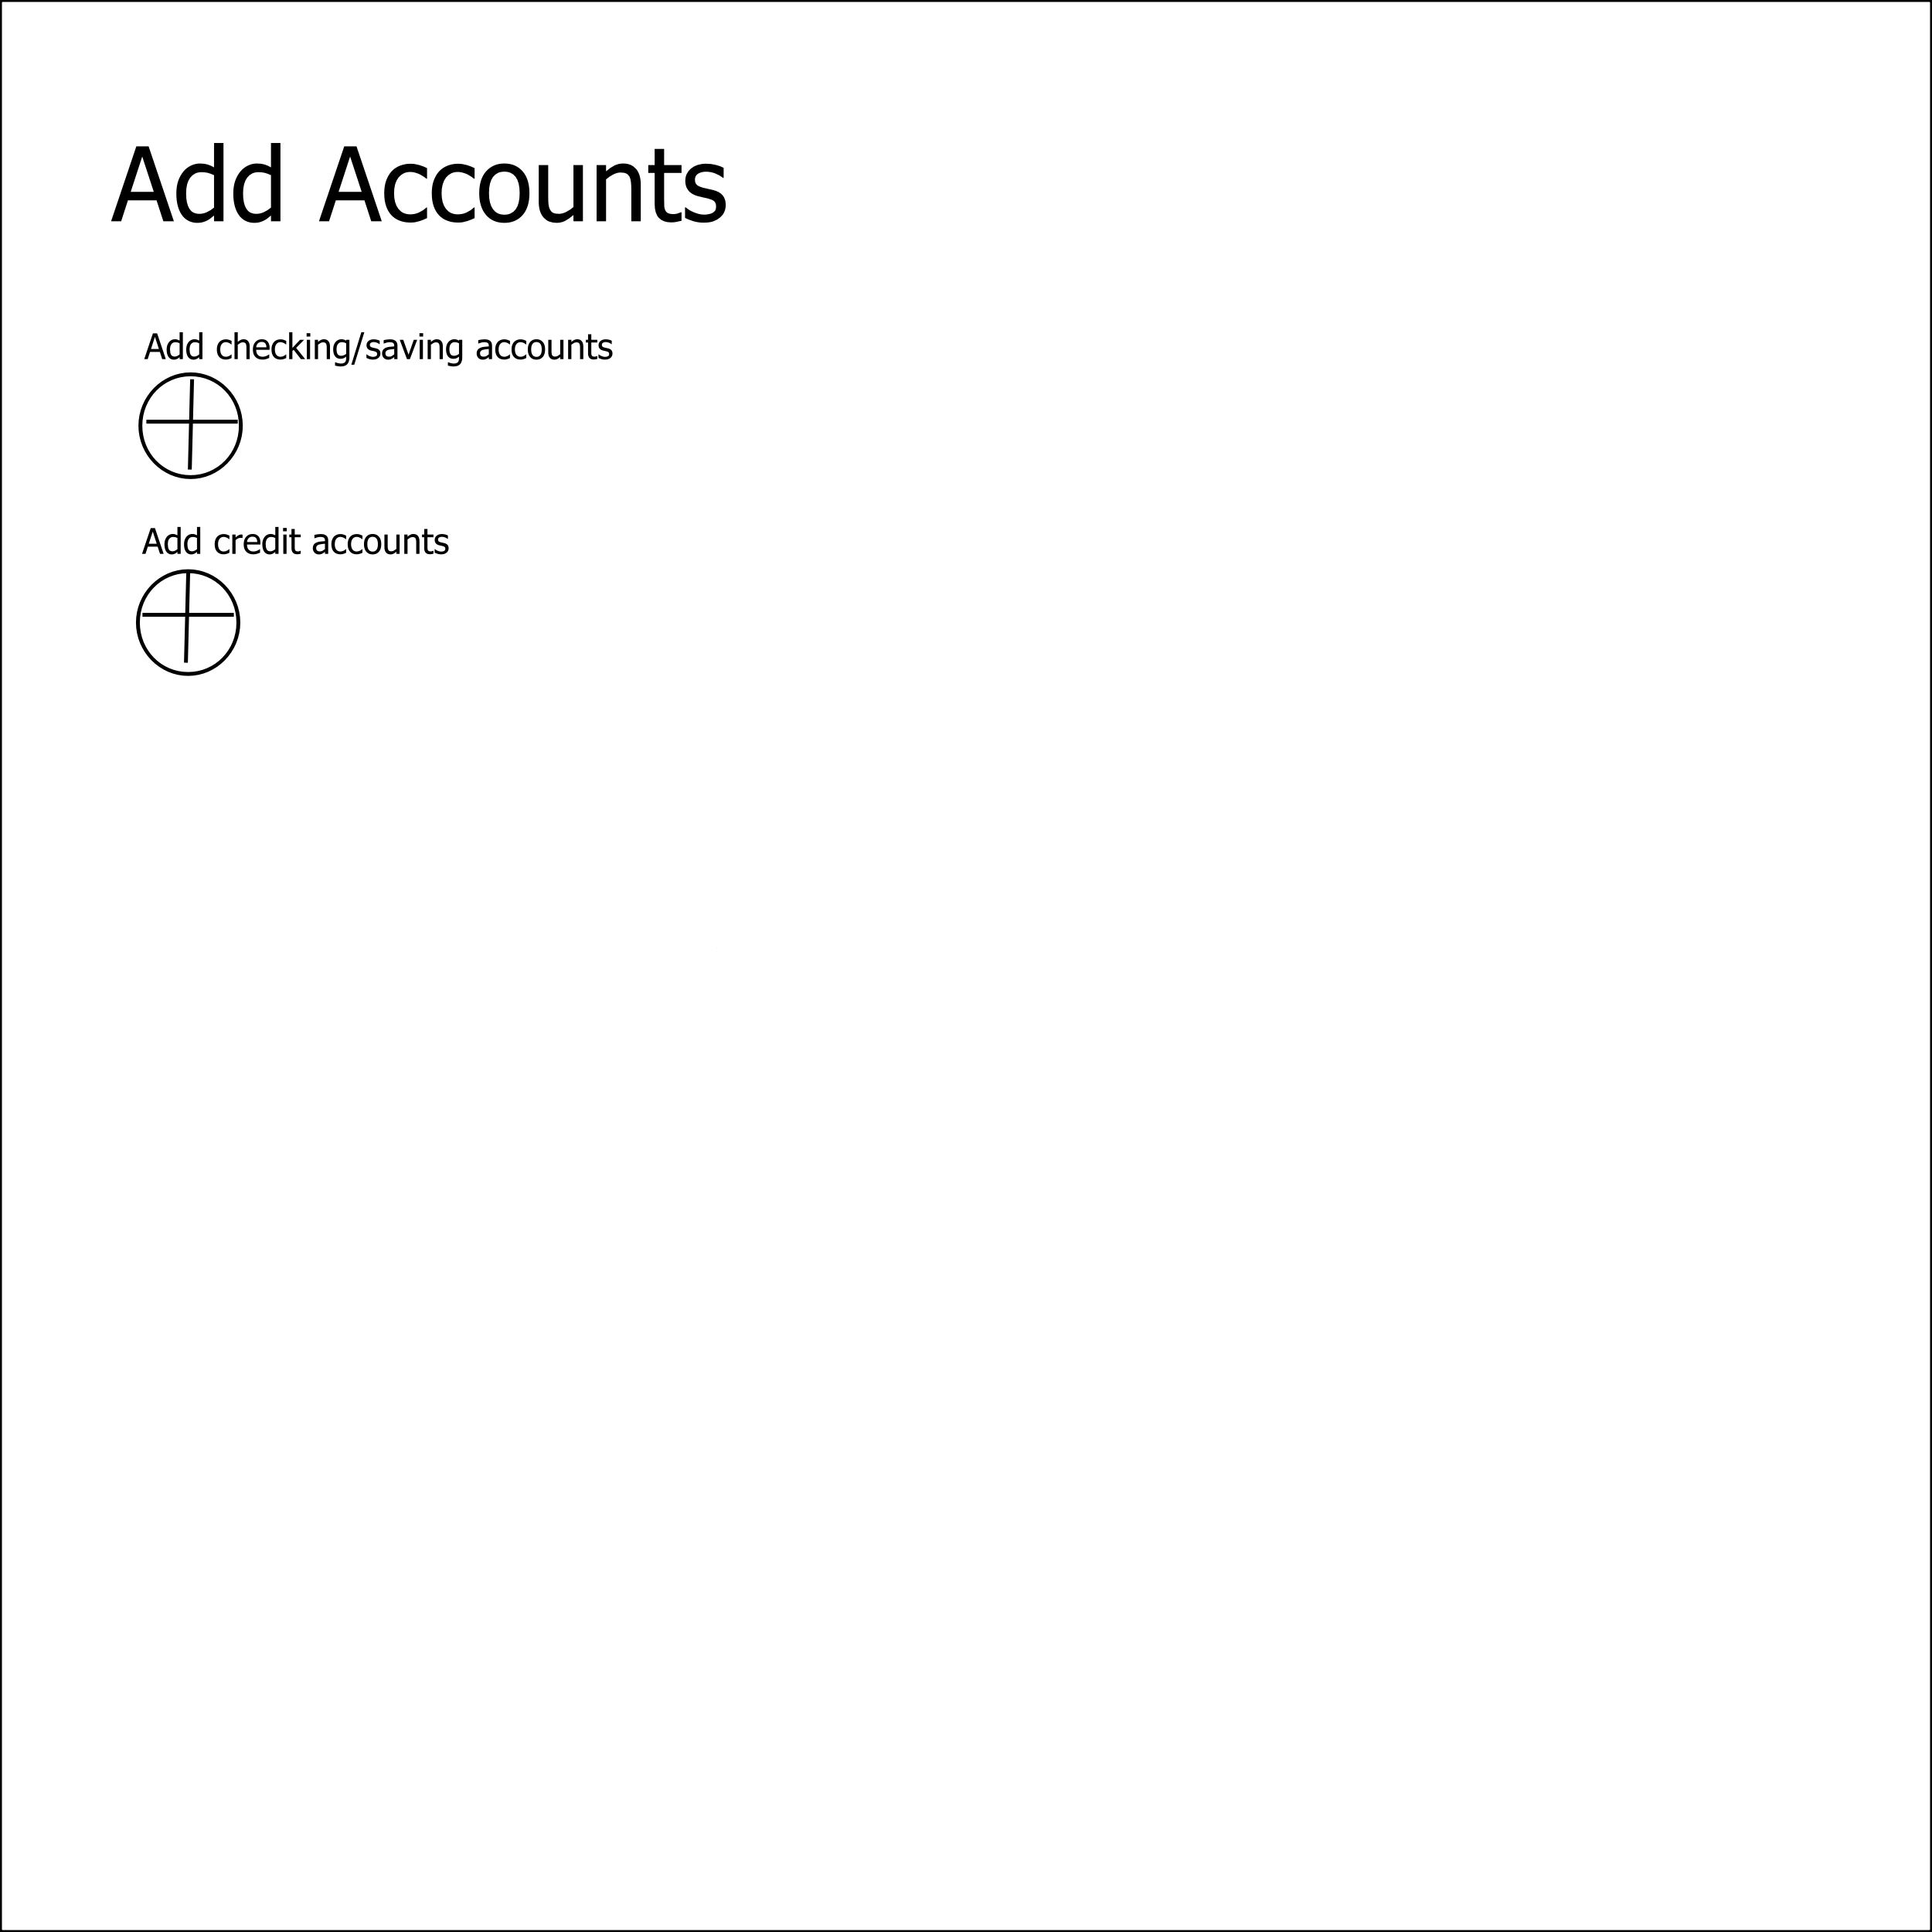
\includegraphics[width=3in]{first_time_add_bank_accounts.jpg}\\
The final step of account creation is adding the users financial accounts.\\


\subsubsection{Budget View}
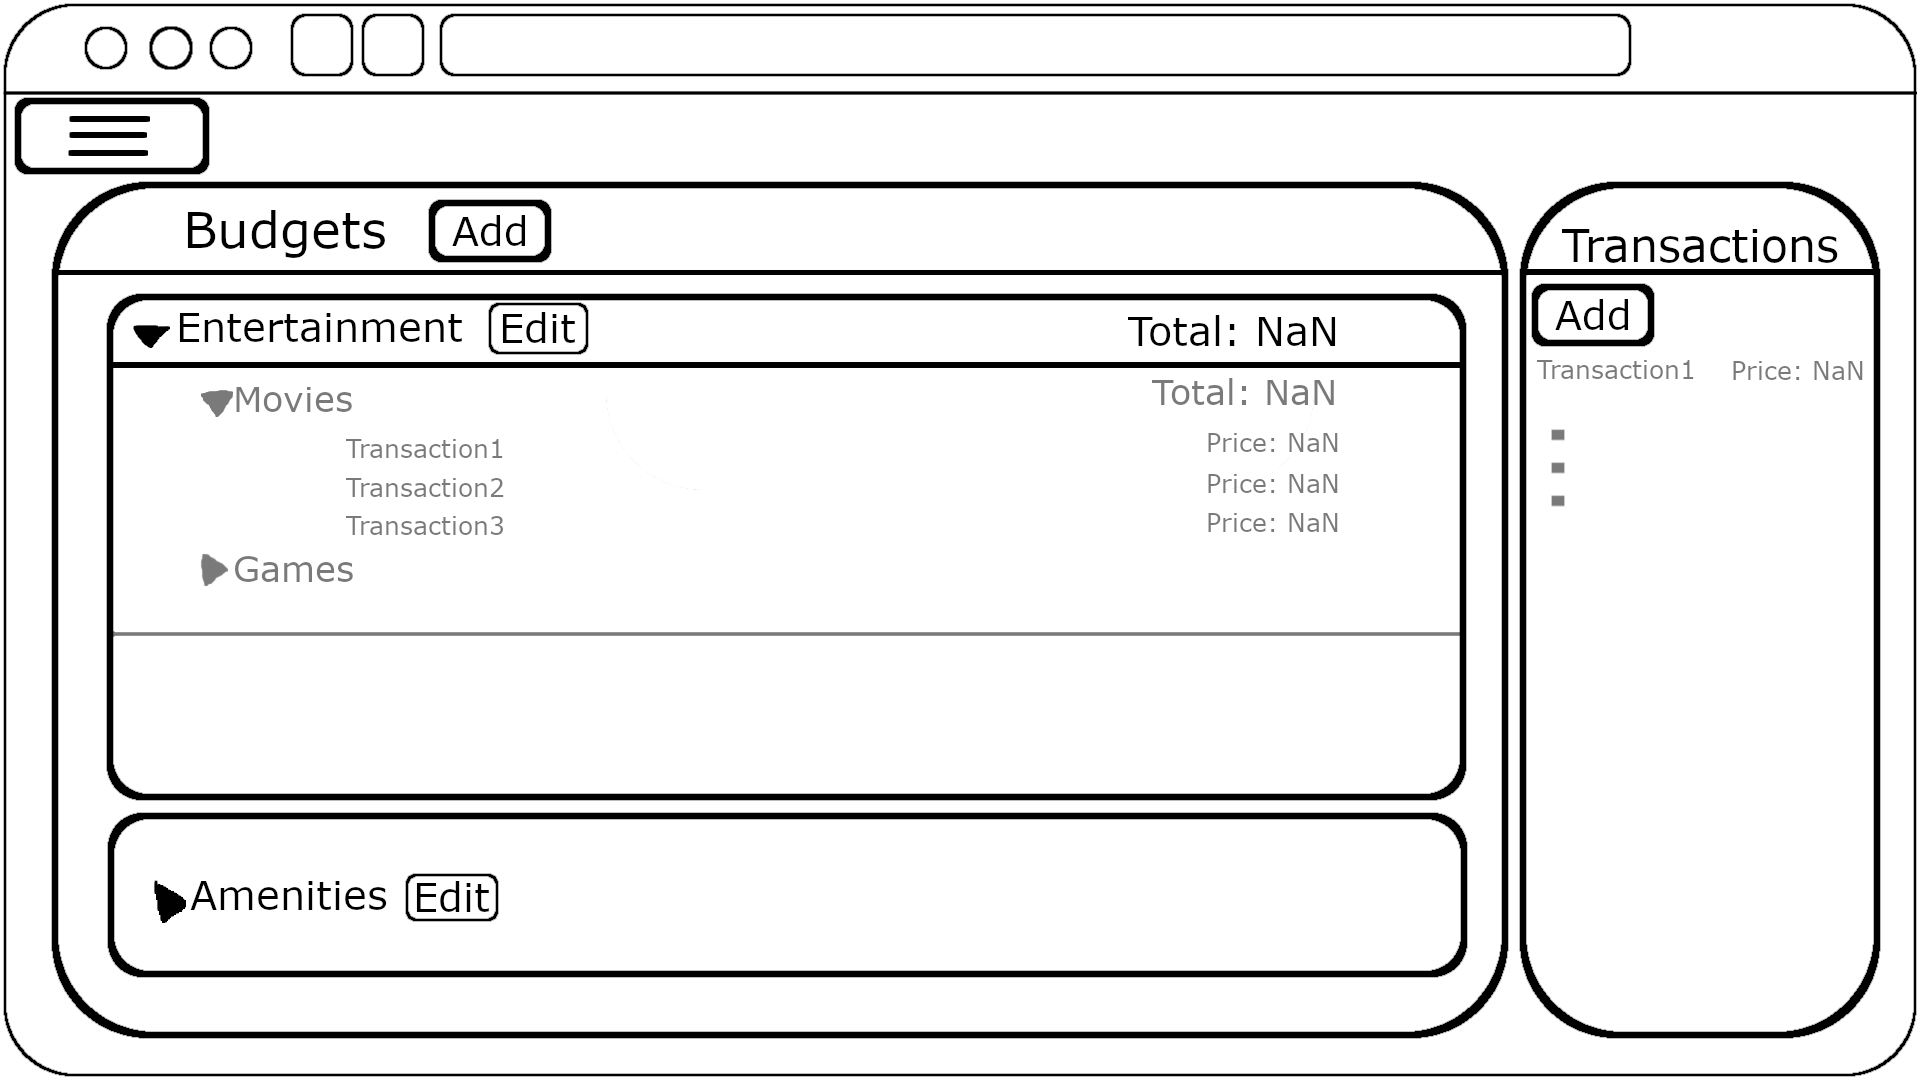
\includegraphics[width=3in]{BudgetPagePersonal.png}
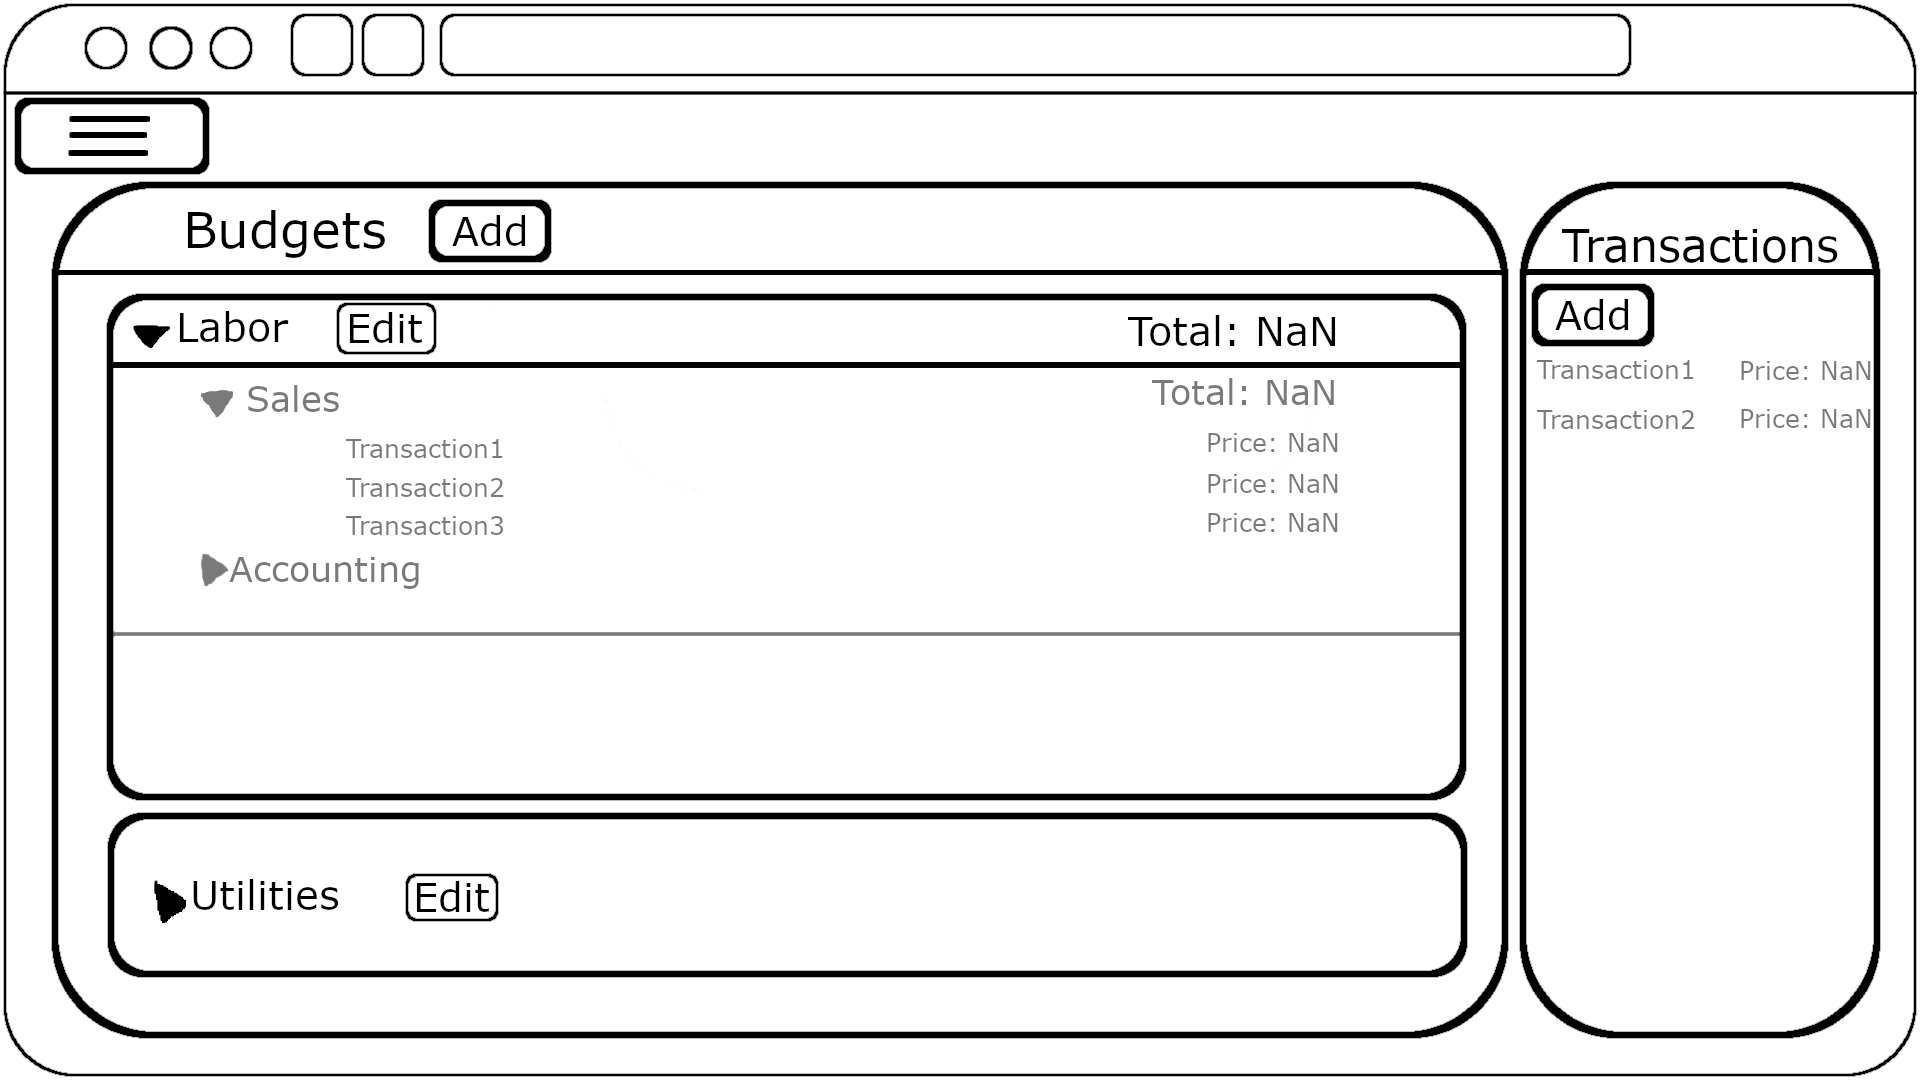
\includegraphics[width=3in]{BudgetPageBusiness.png}\\
This is the page users will land on when they get done with registering or when they sign in. On the left is the personal version and on the right is the business version. The main difference between the two are the default tags. Here they can add and edit their budgets and add transactions.\\

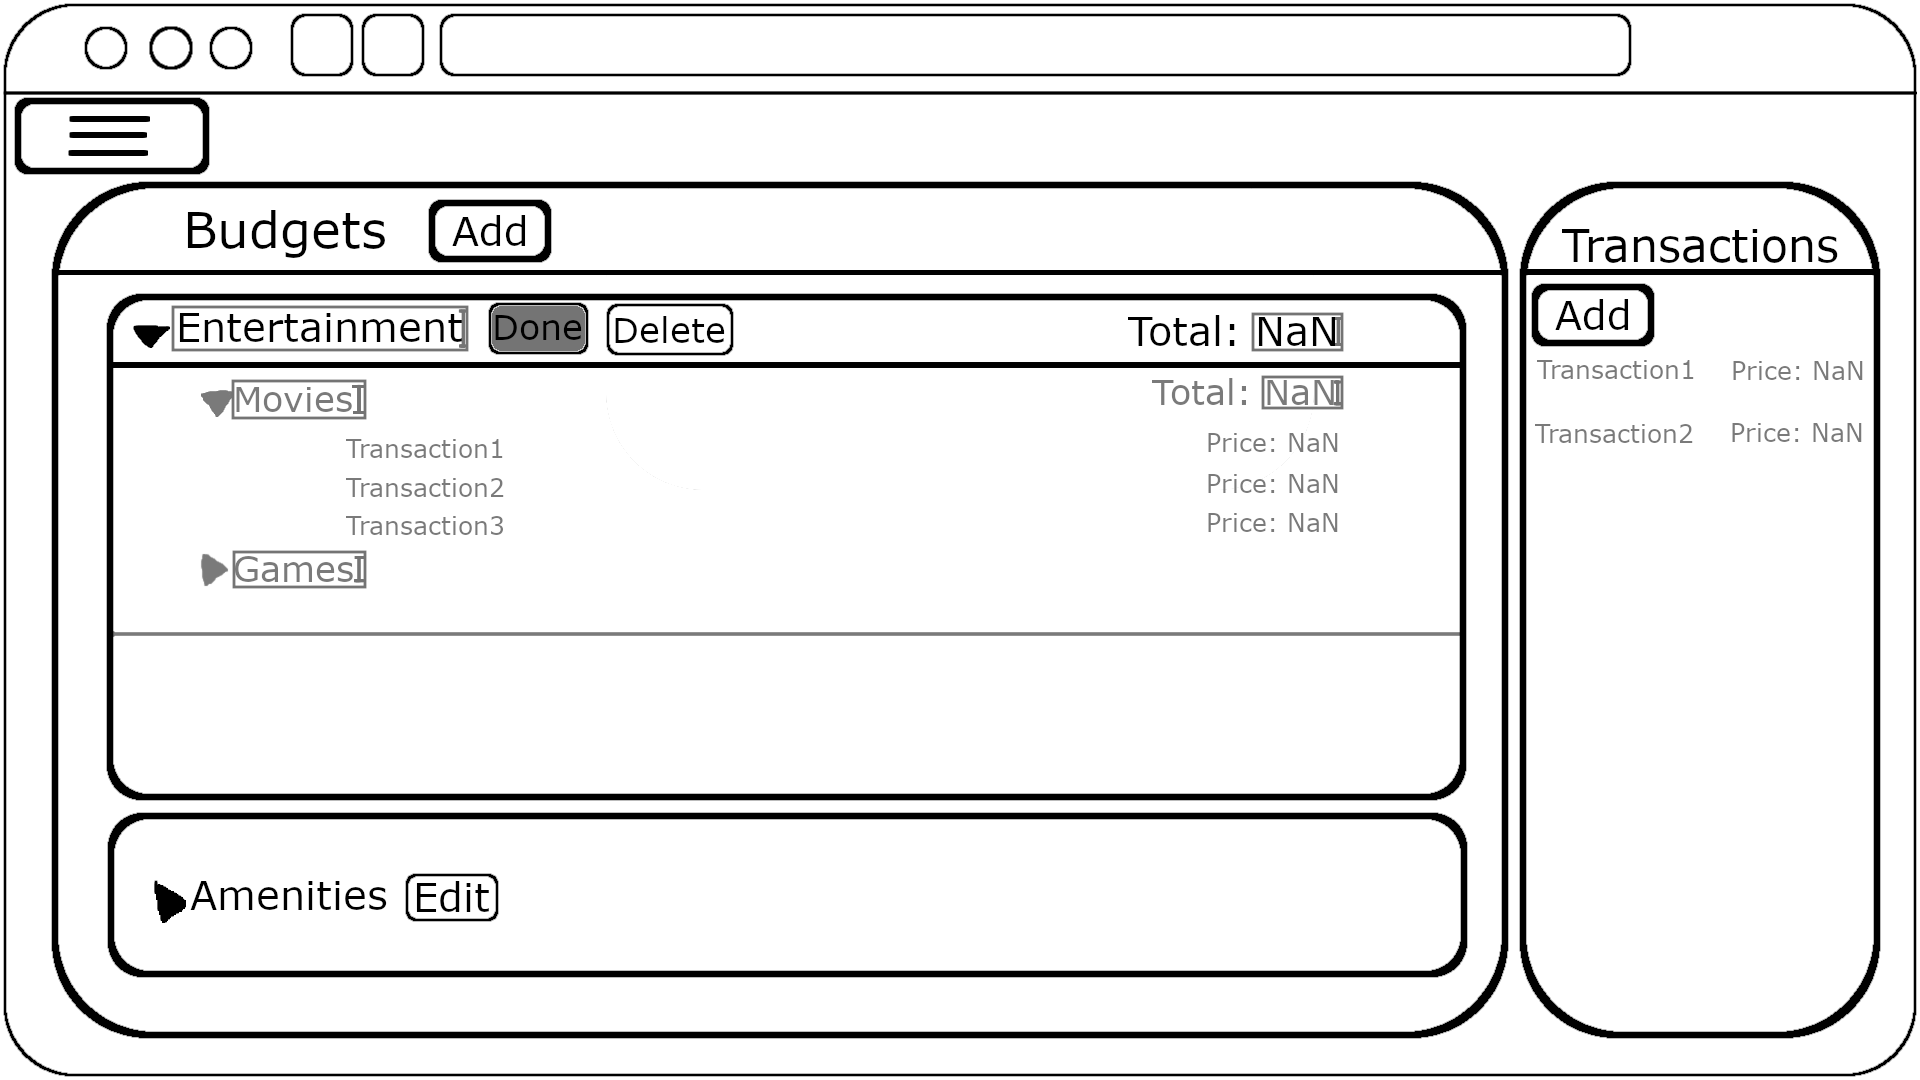
\includegraphics[width=3in]{BudgetPageEditPushed.png}
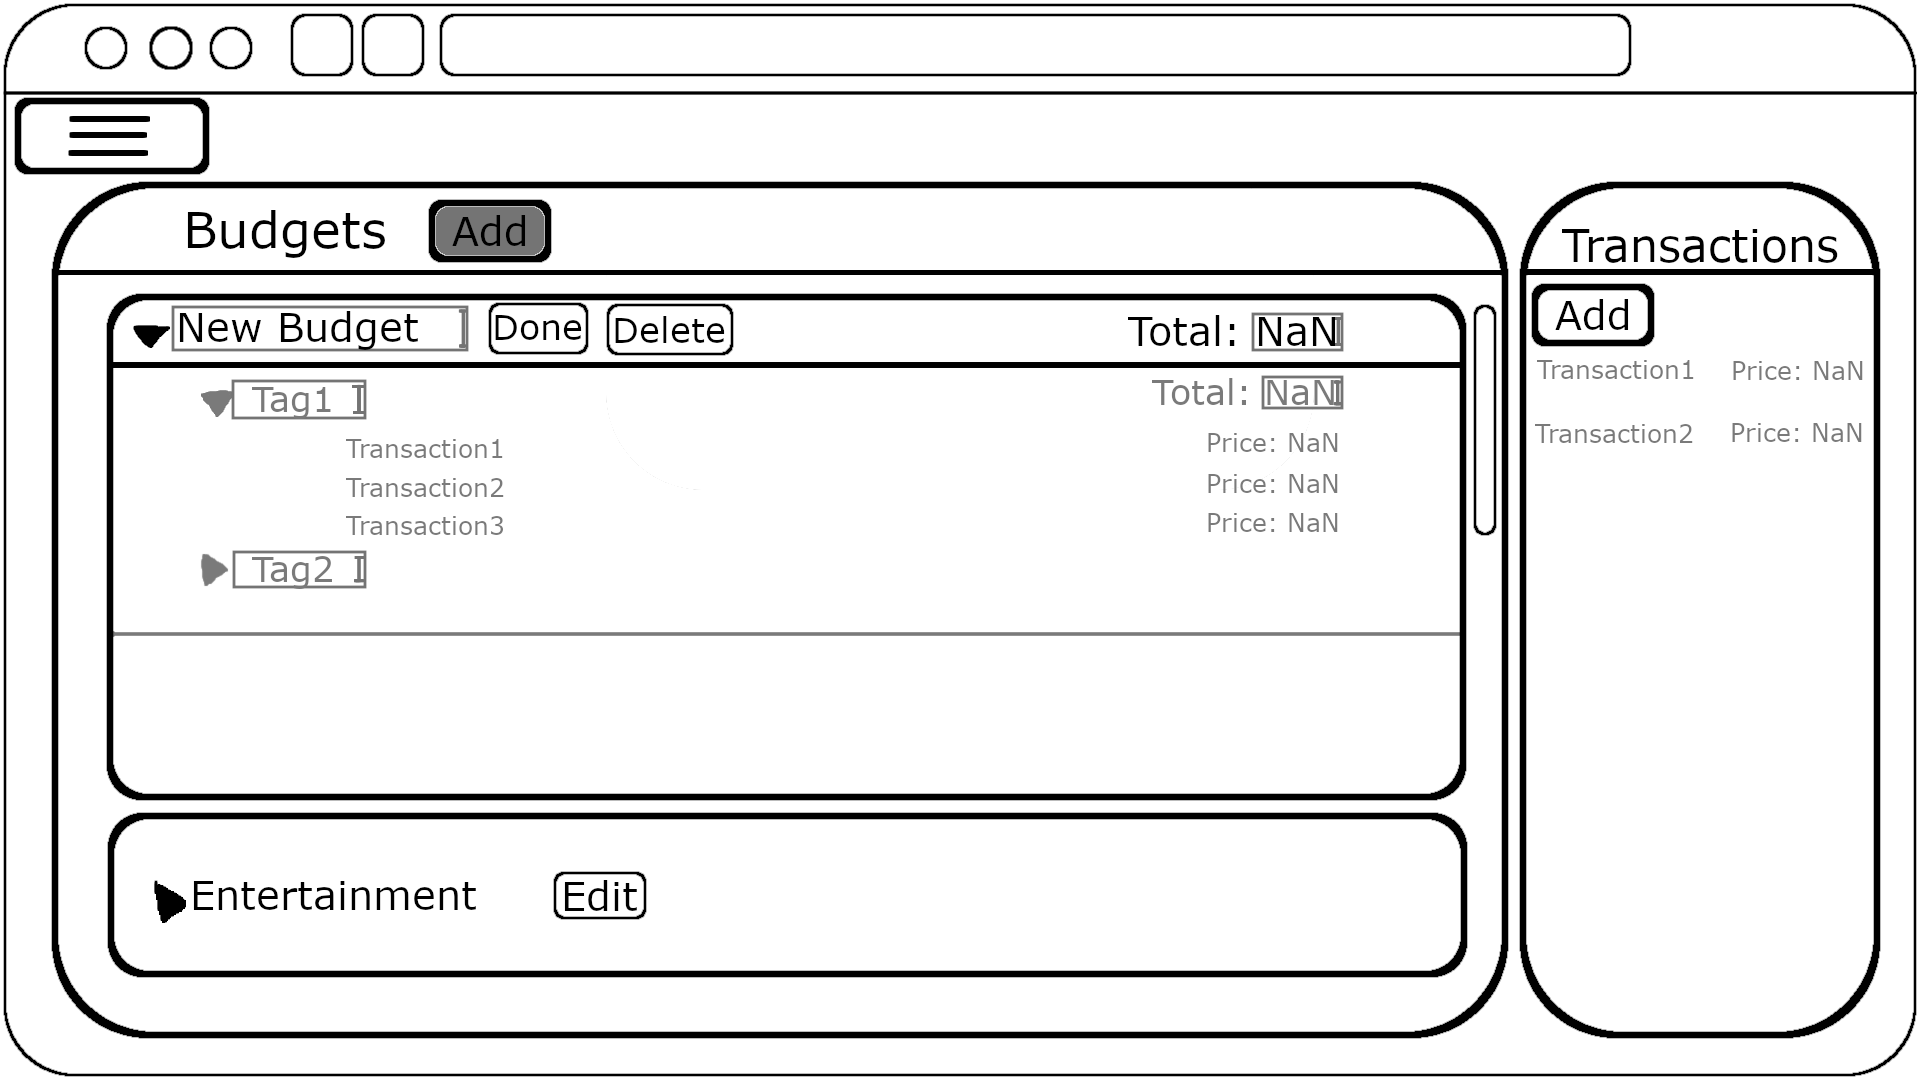
\includegraphics[width=3in]{BudgetPageAddPushed.png}\\
When the edit button (next to a budget) is pushed, the fields for the name of the budget, the tags, and the totals become editable. When the add button is pushed a new budget is added to the top of the budget view and the fields are editable by default. When the done button is pushed the fields become finalized.\\

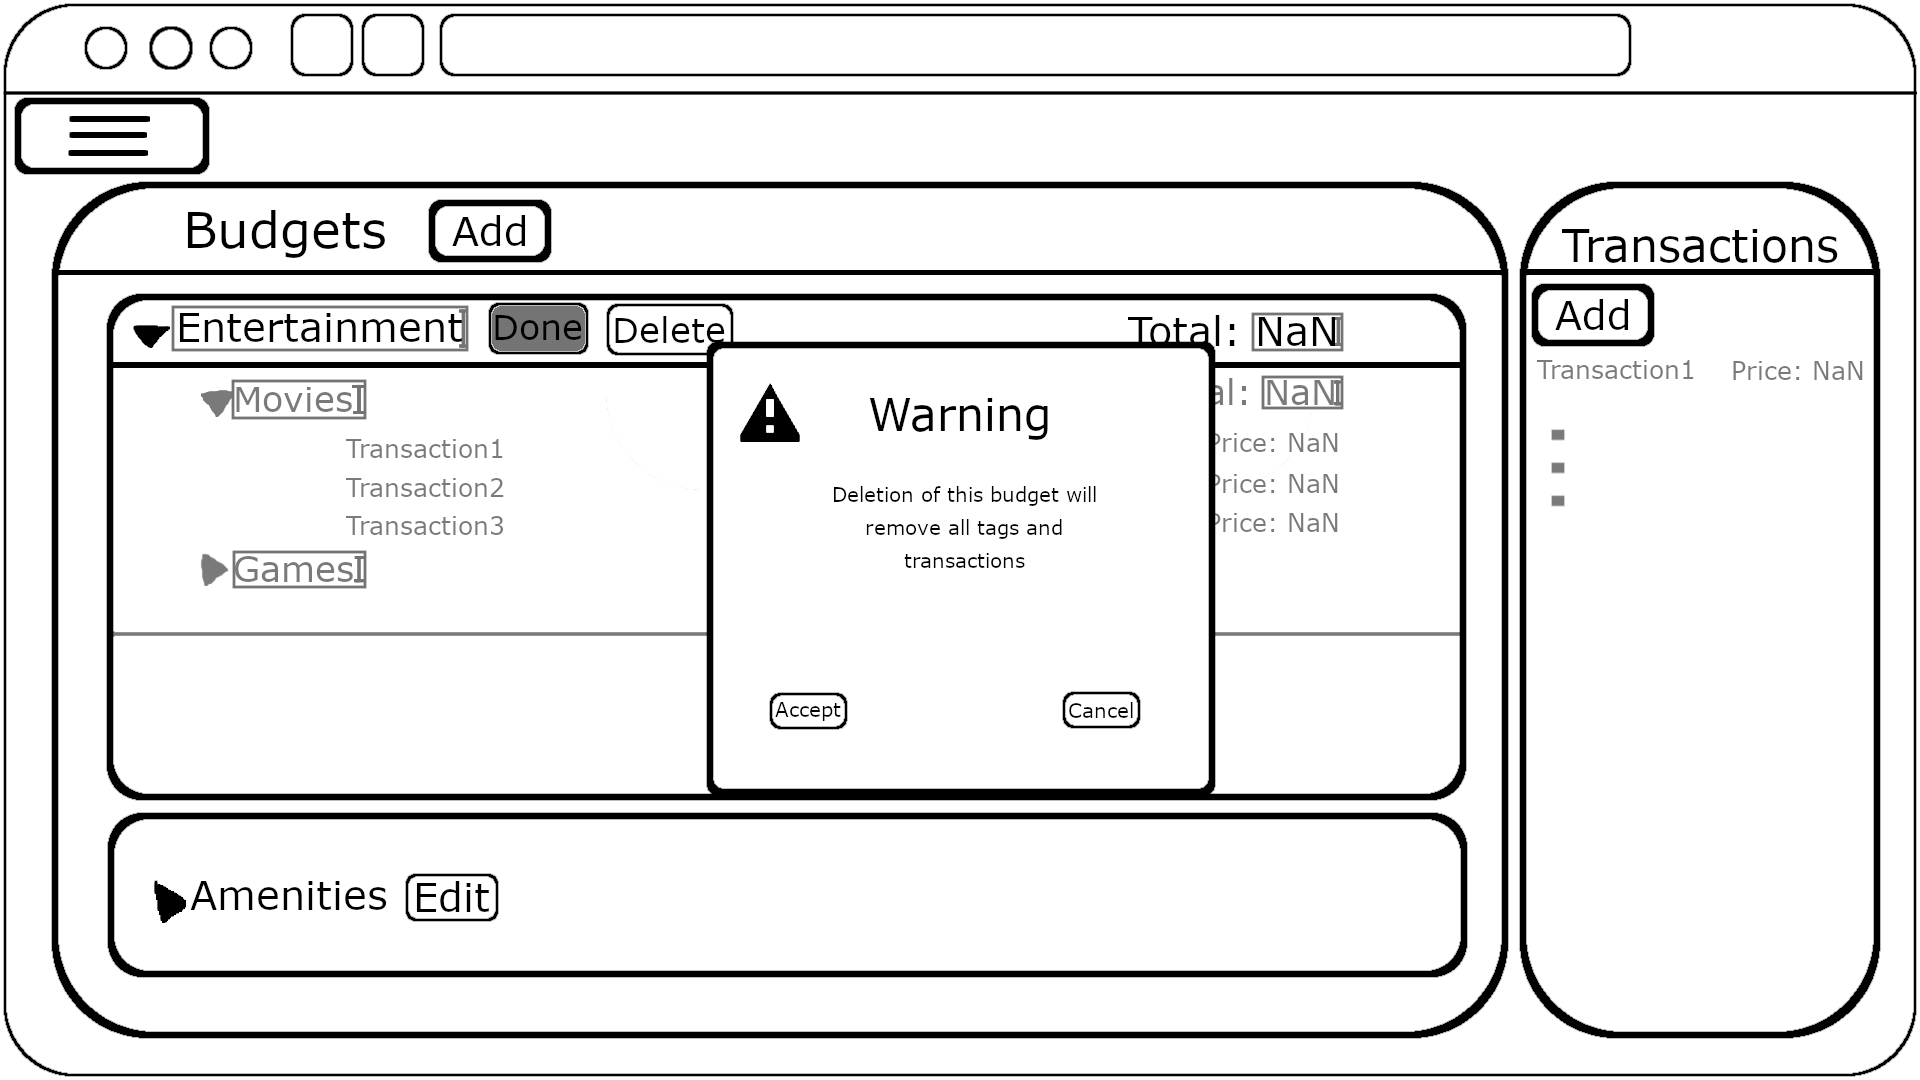
\includegraphics[width=3in]{BudgetPageWarning.png}\\
When the delete button is pushed a warning will be shown to the user. If the user accepts then the budget, along with it's tags, are deleted. Transactions are moved to a budget called "other".\\

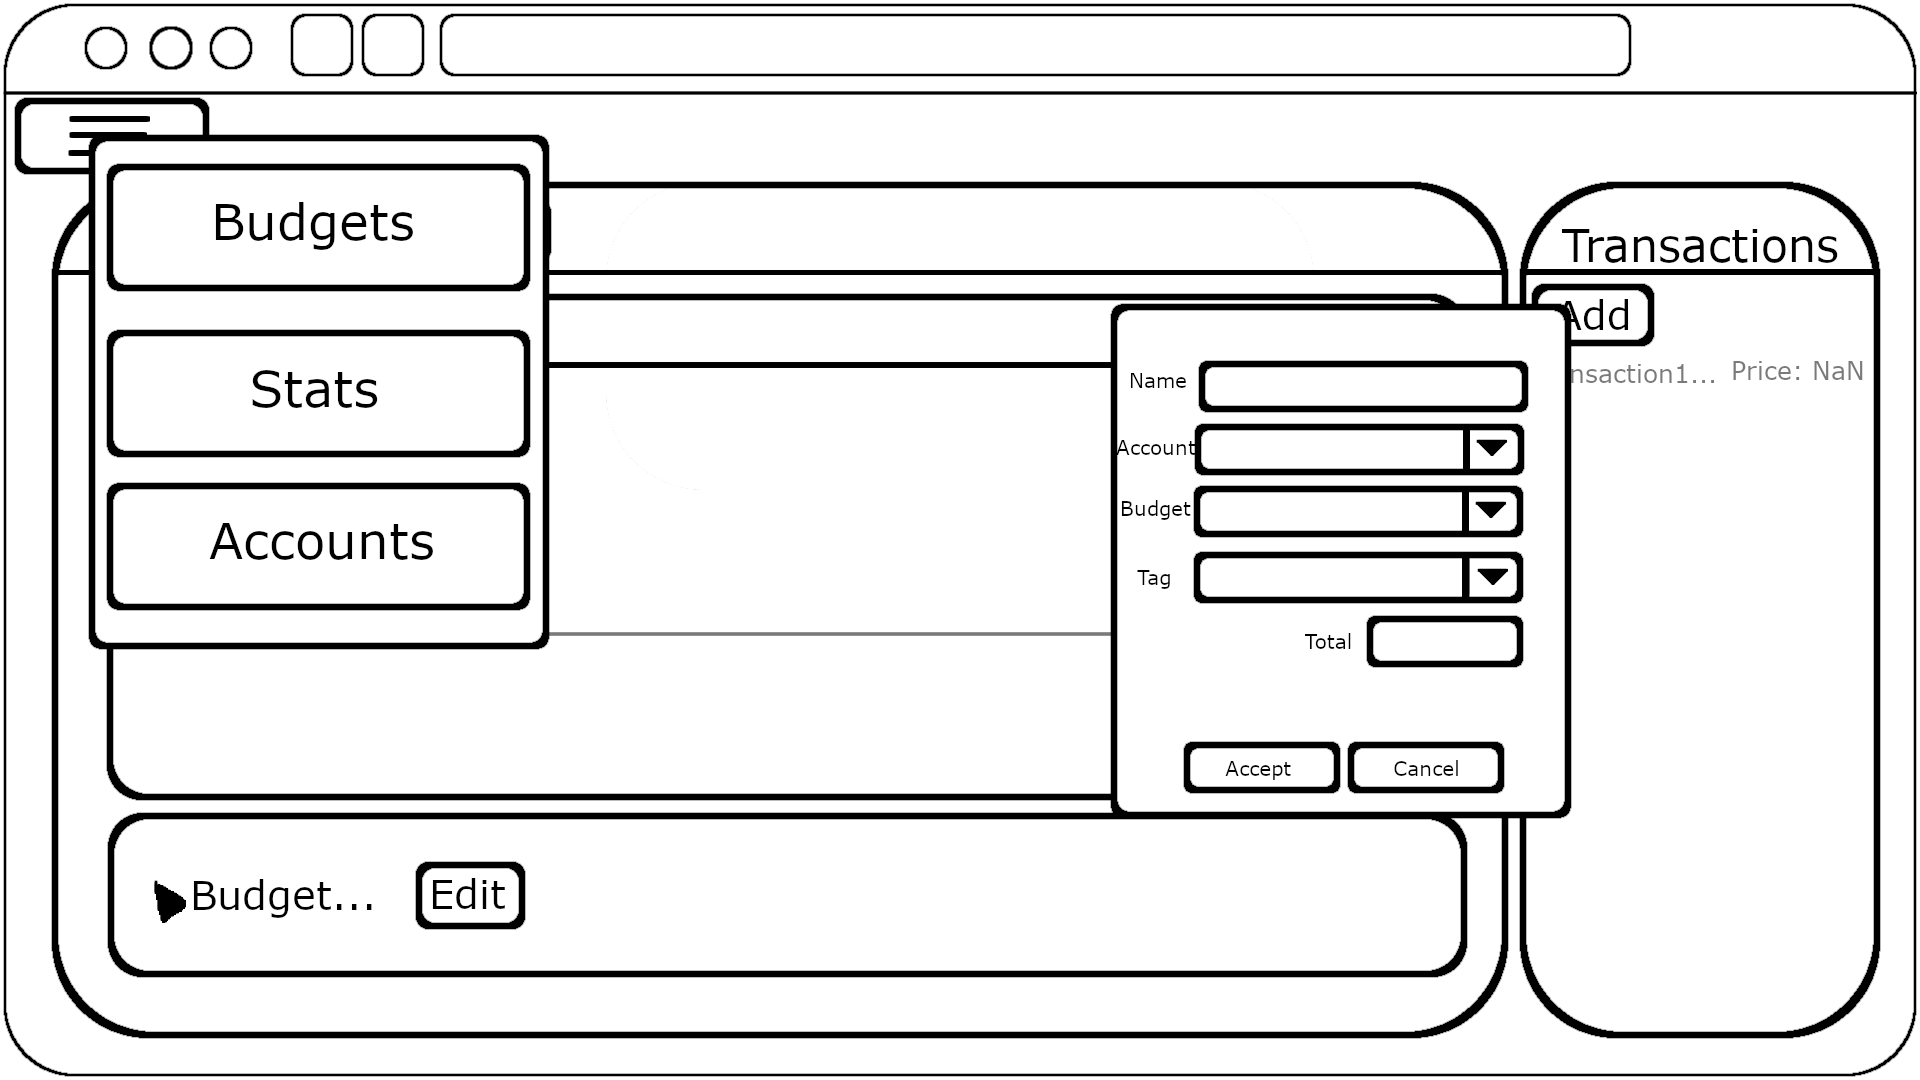
\includegraphics[width=3in]{BudgetPageWithMenu.png}\\
This shows the various popups that the page will have. Pushing the add transaction button will prompt the user to add in a transaction. Pushing the menu in the top left will show the user different pages they can go to.\\

\subsubsection{Account View}
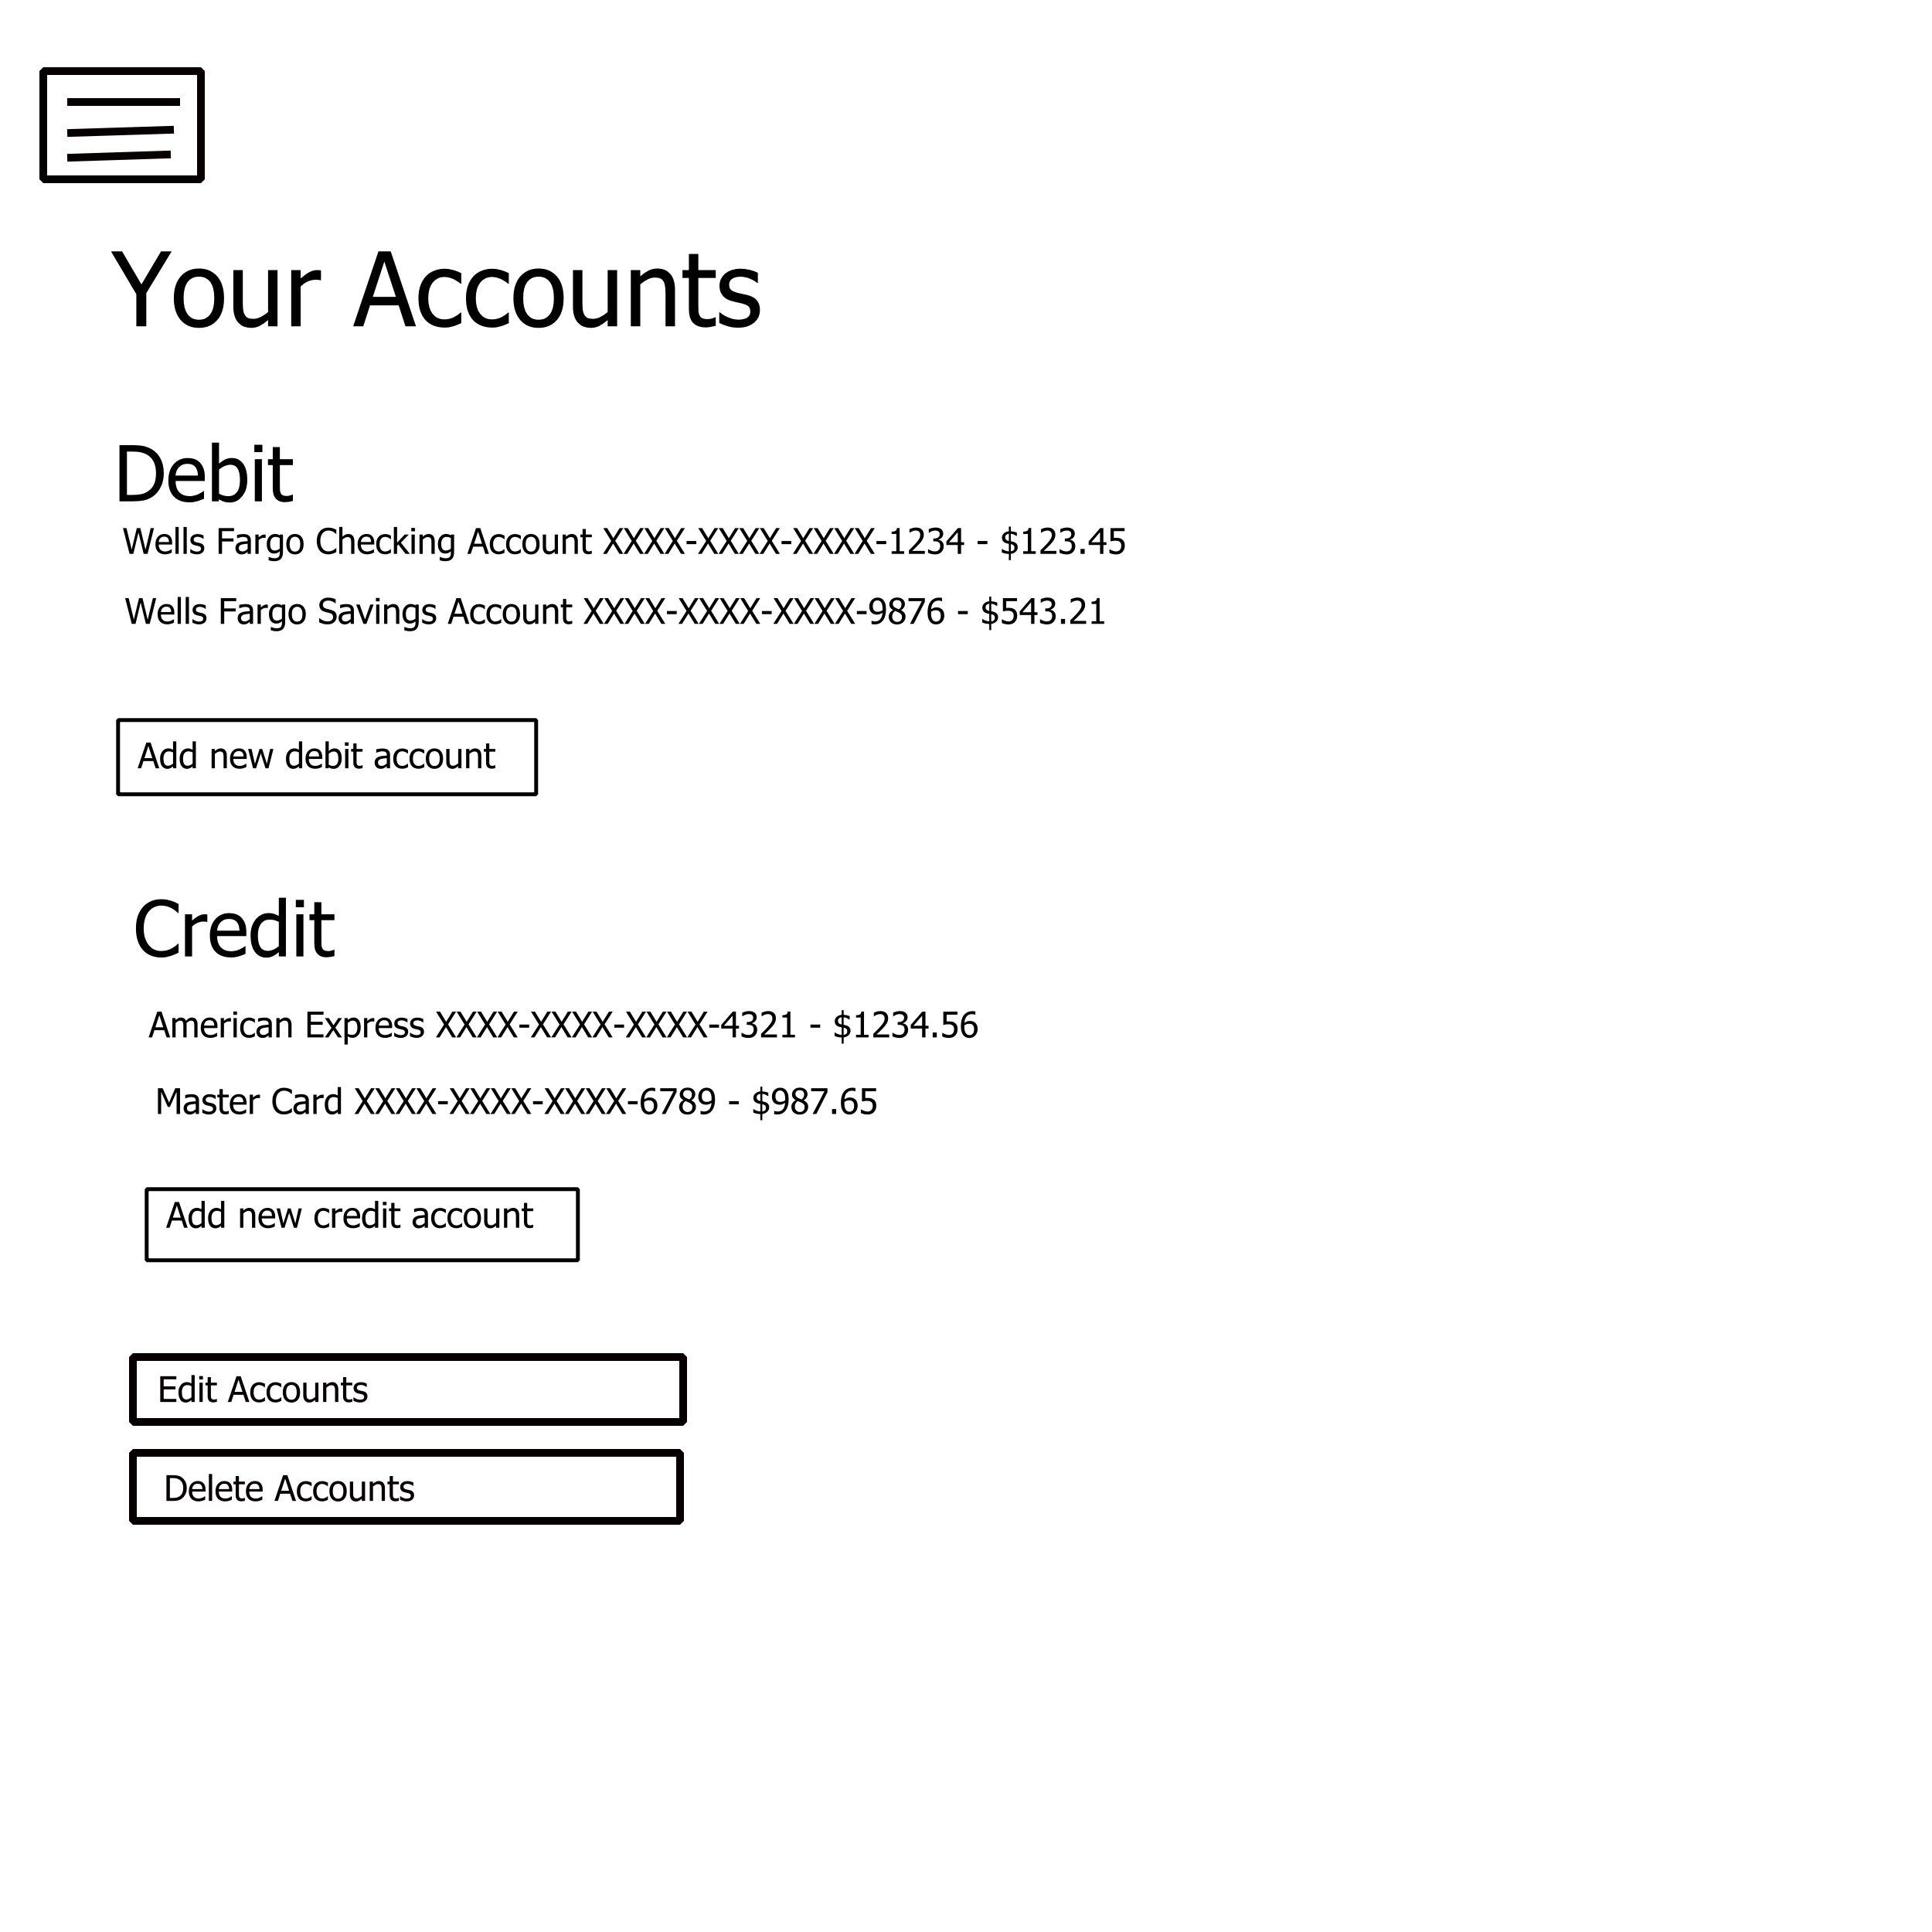
\includegraphics[width=3in]{your_accounts_page.jpg}\\
The users can view their accounts in aggregate and also add new accounts if they are created.\\
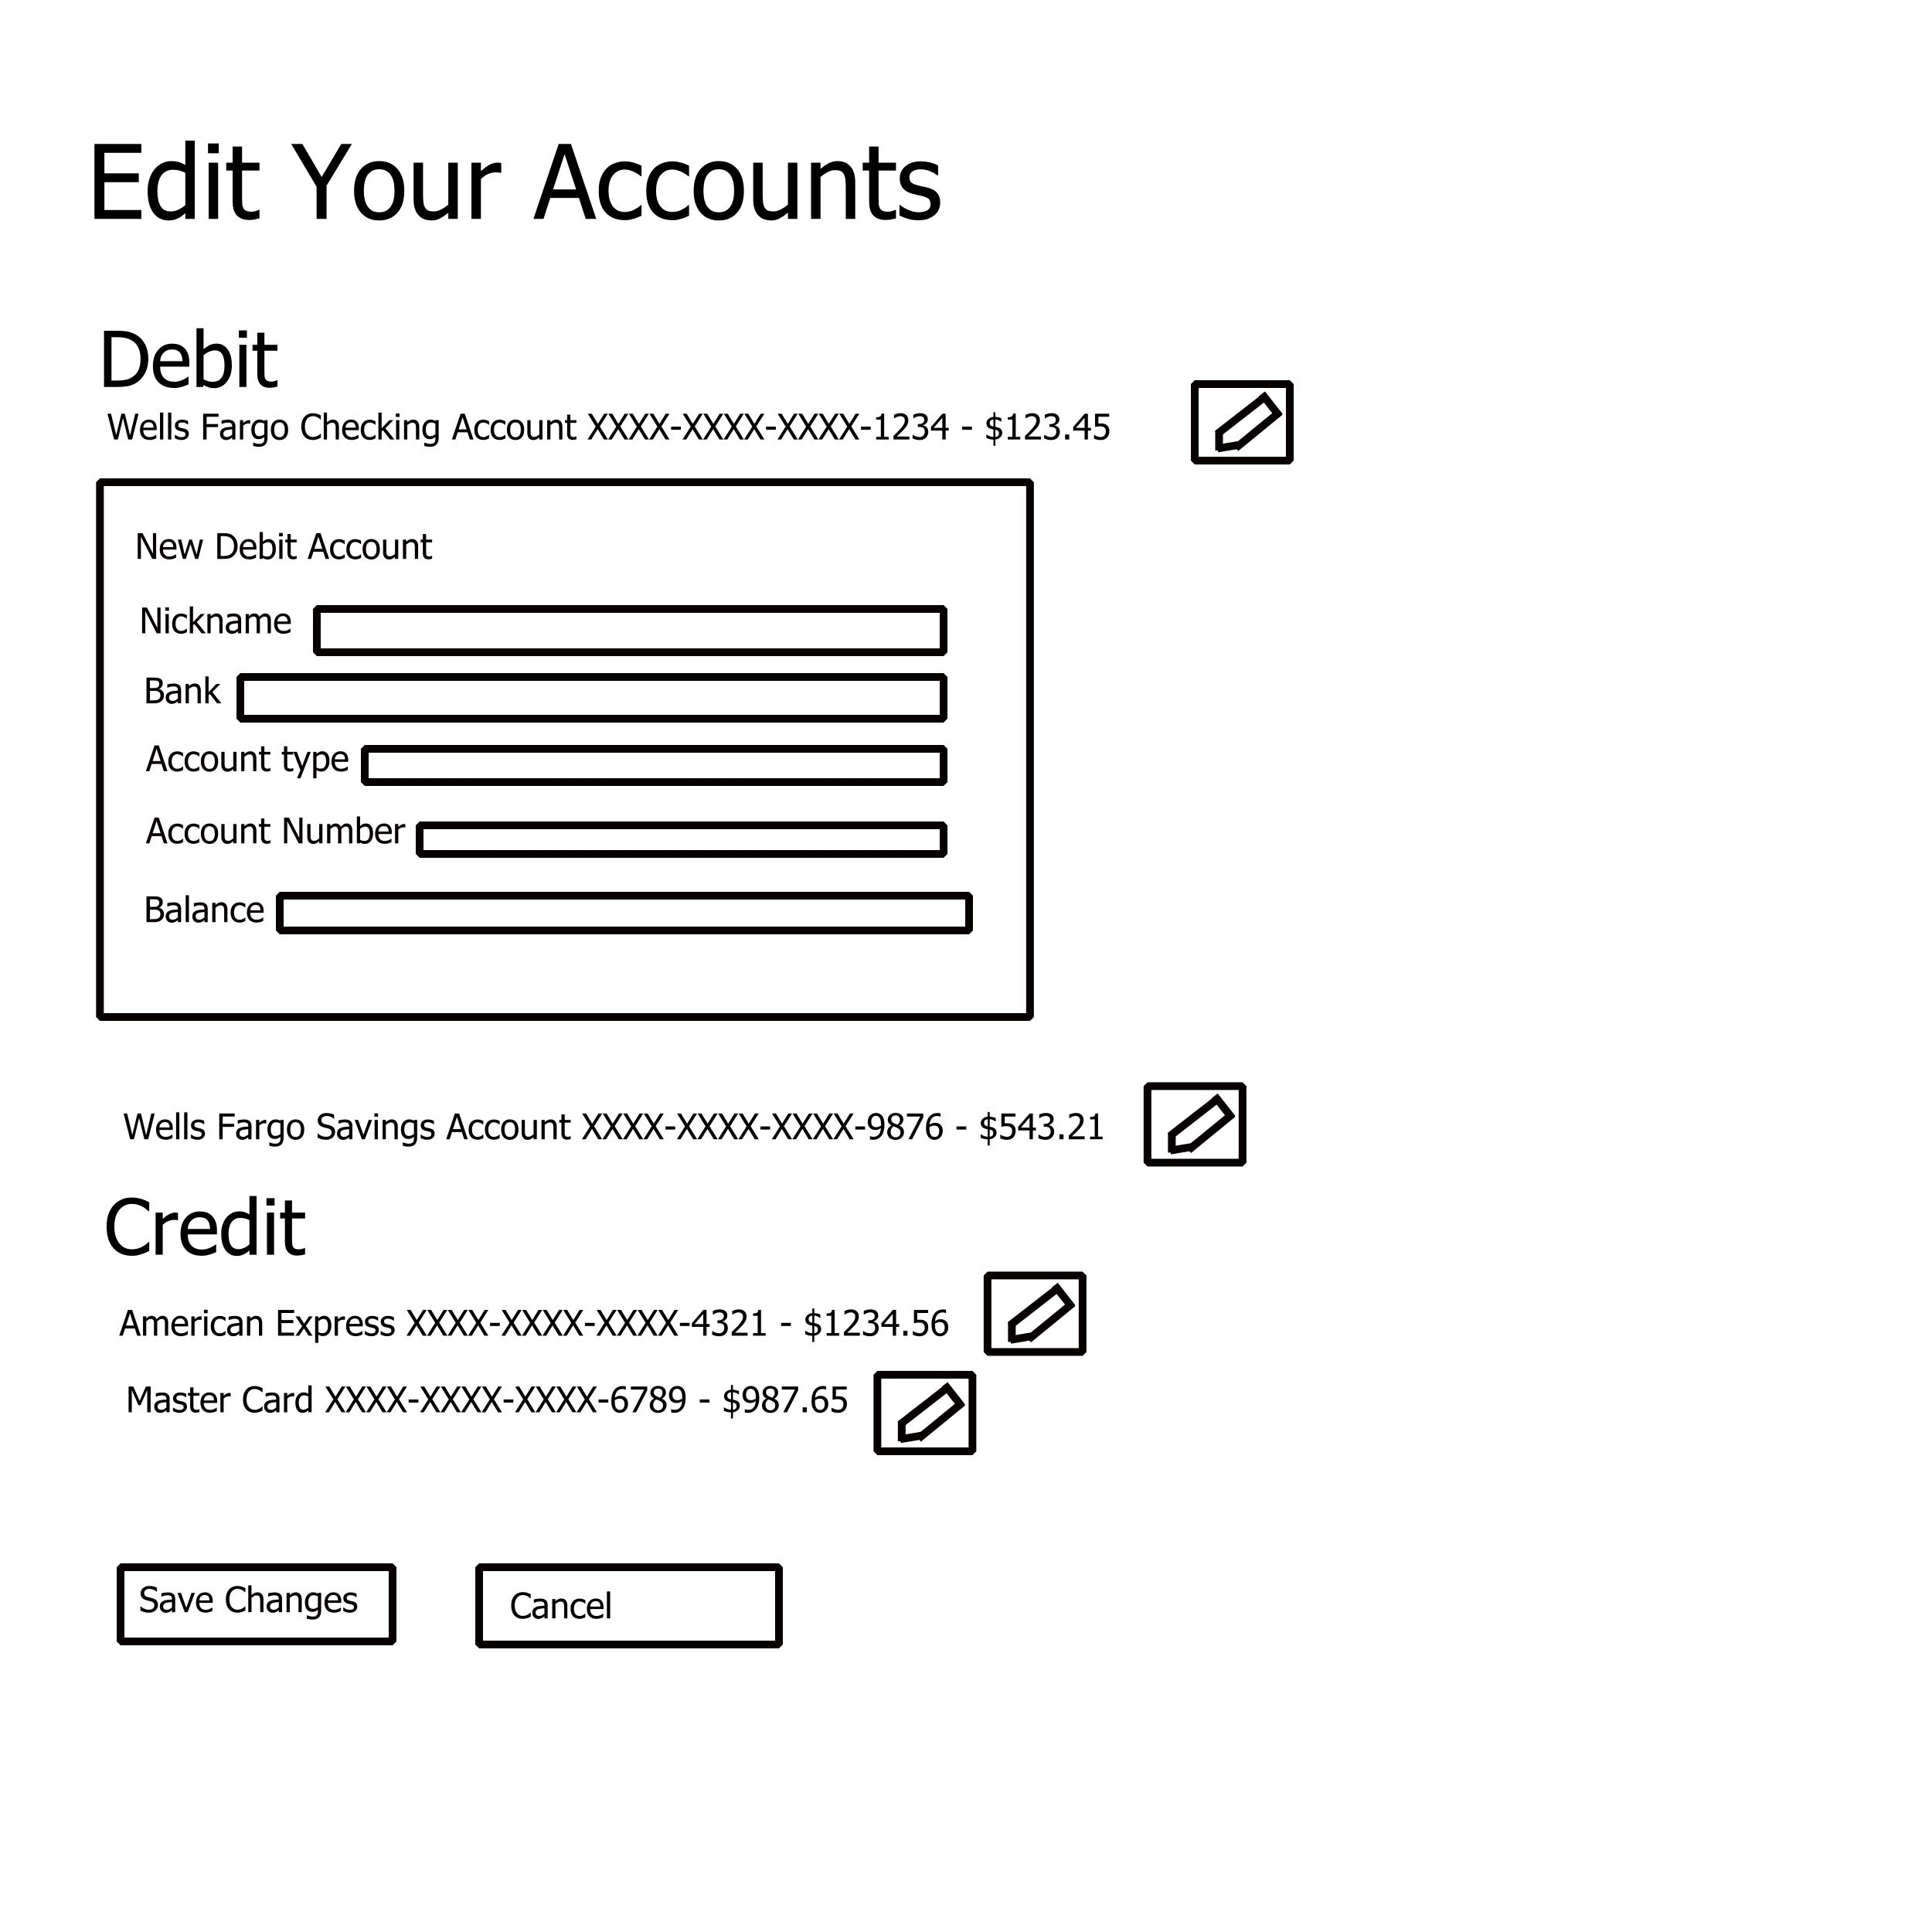
\includegraphics[width=3in]{edit_your_accounts_page.jpg}
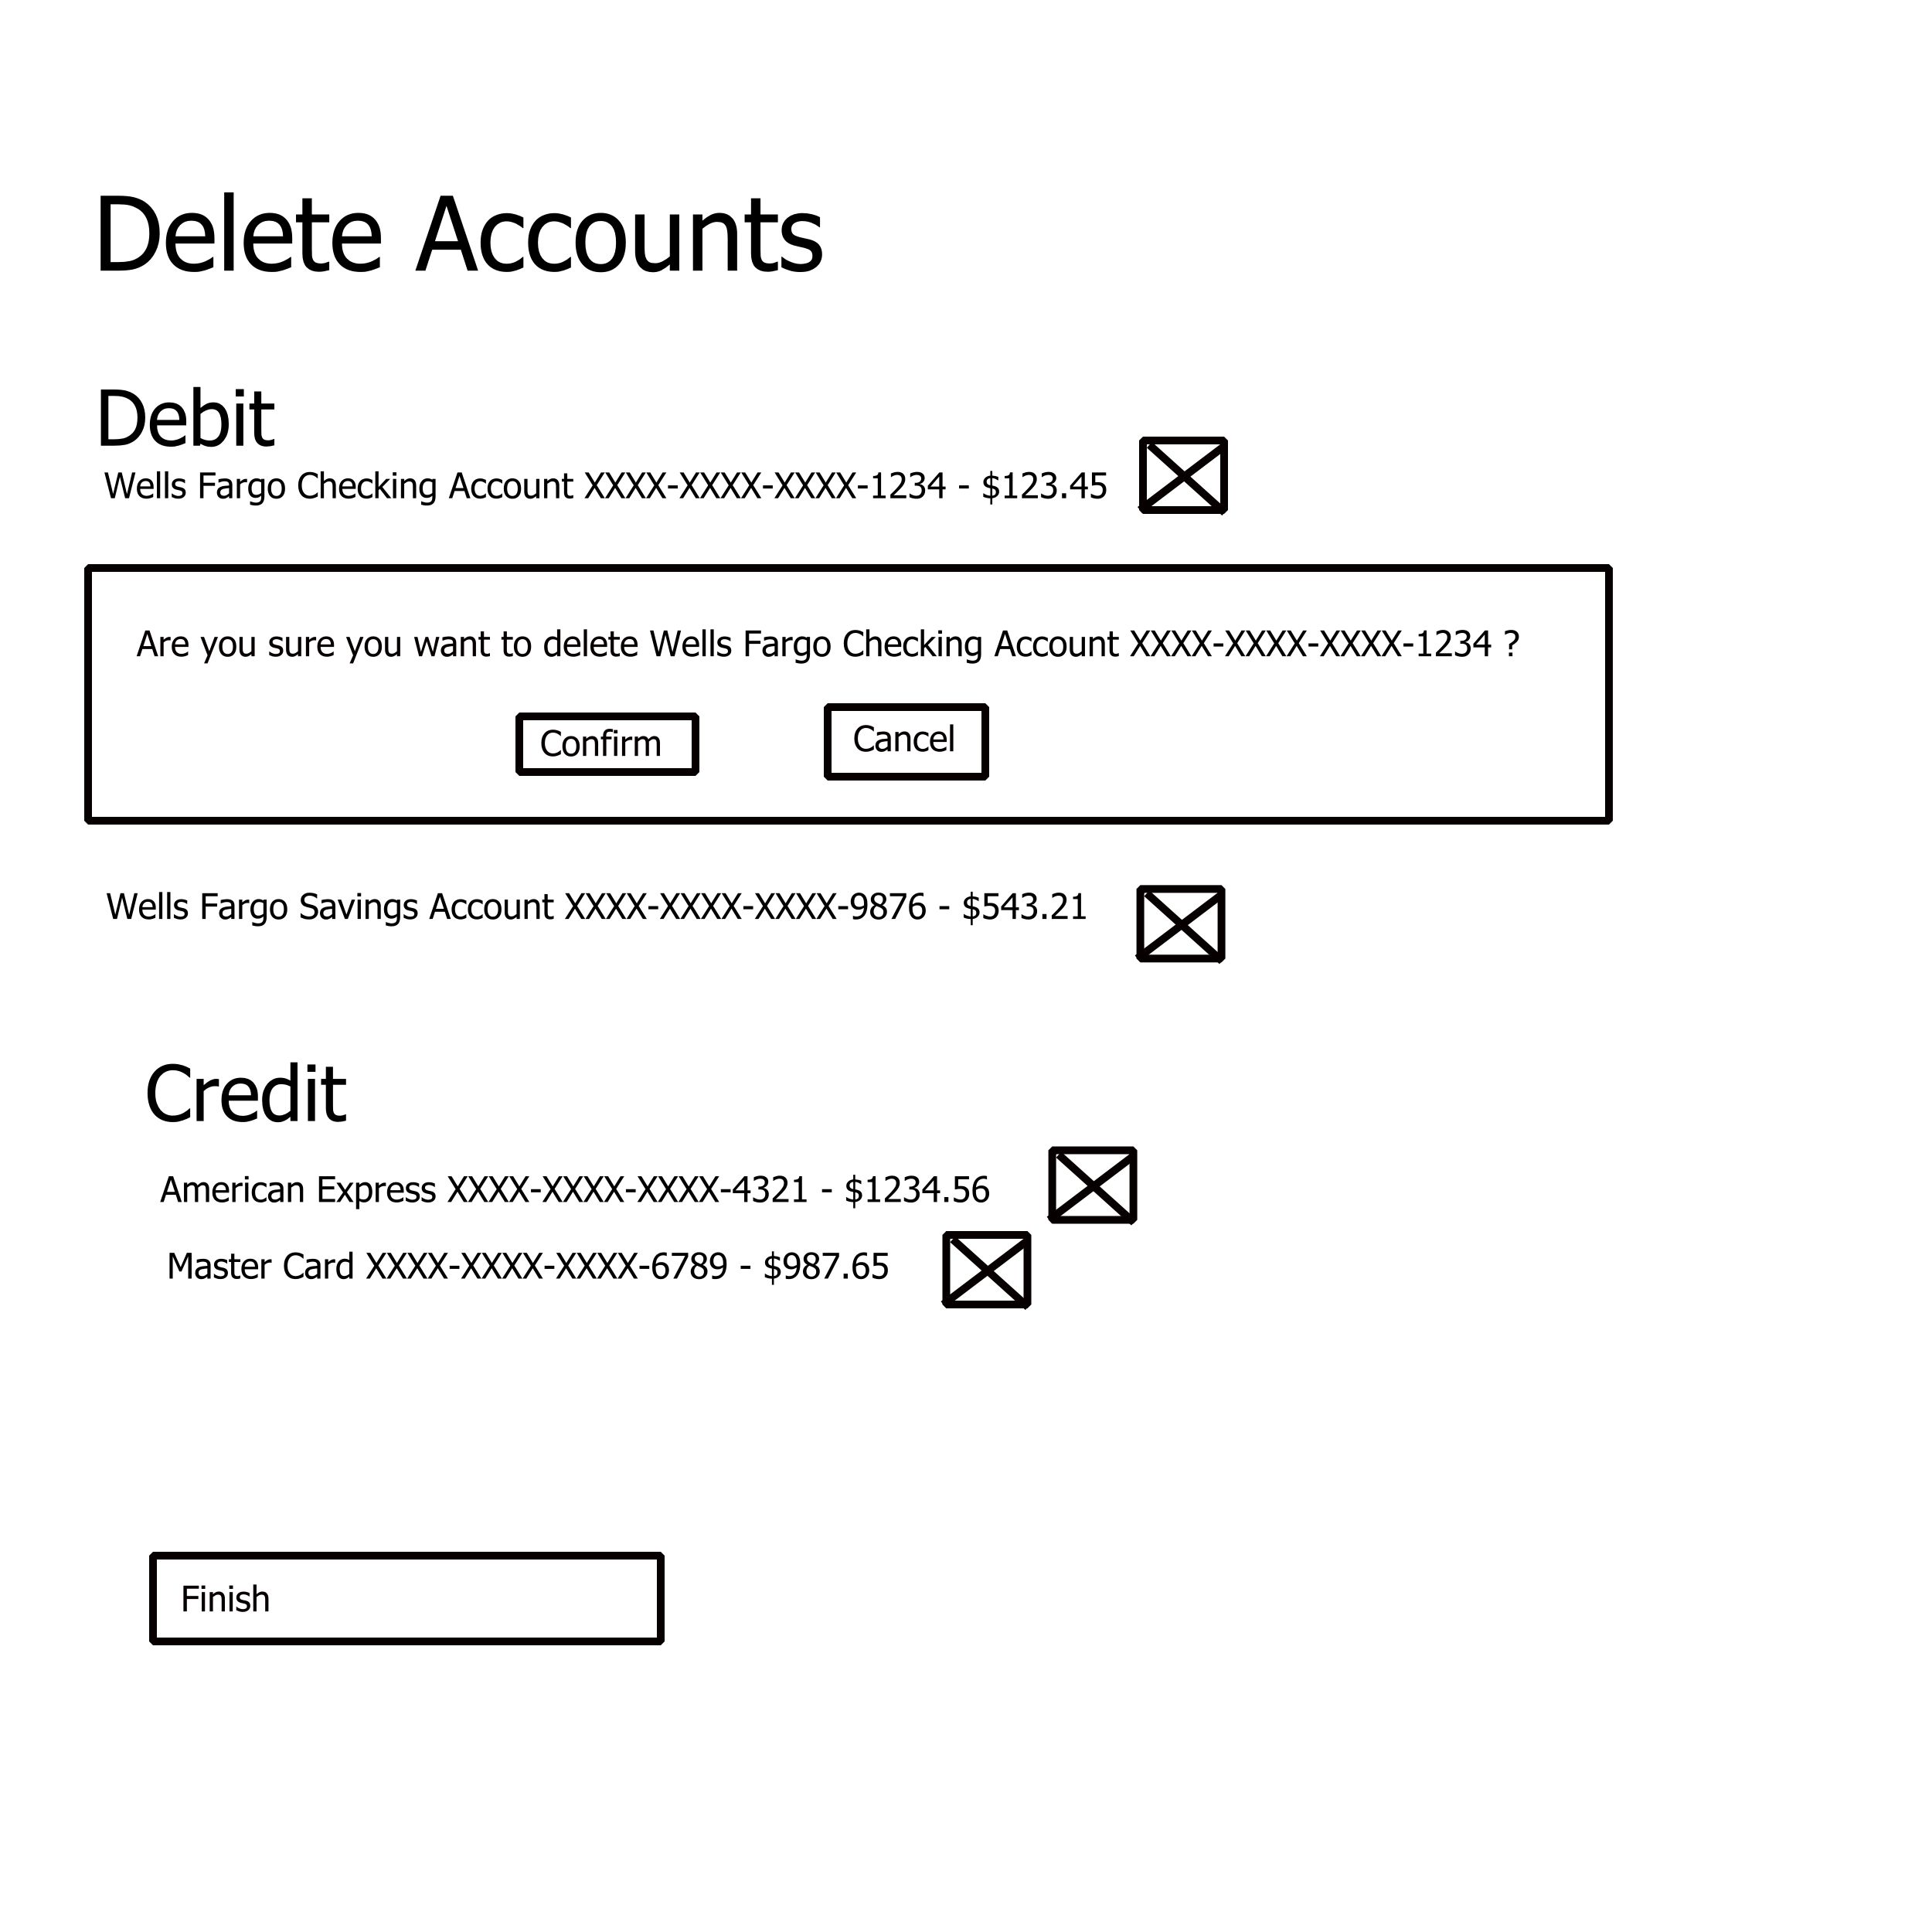
\includegraphics[width=3in]{delete_accounts_page.jpg}\\
From the "Your Accounts" page users can edit an existing account, or delete accounts because they have closed the account or were removed from it.\\

\subsubsection{Stats View}
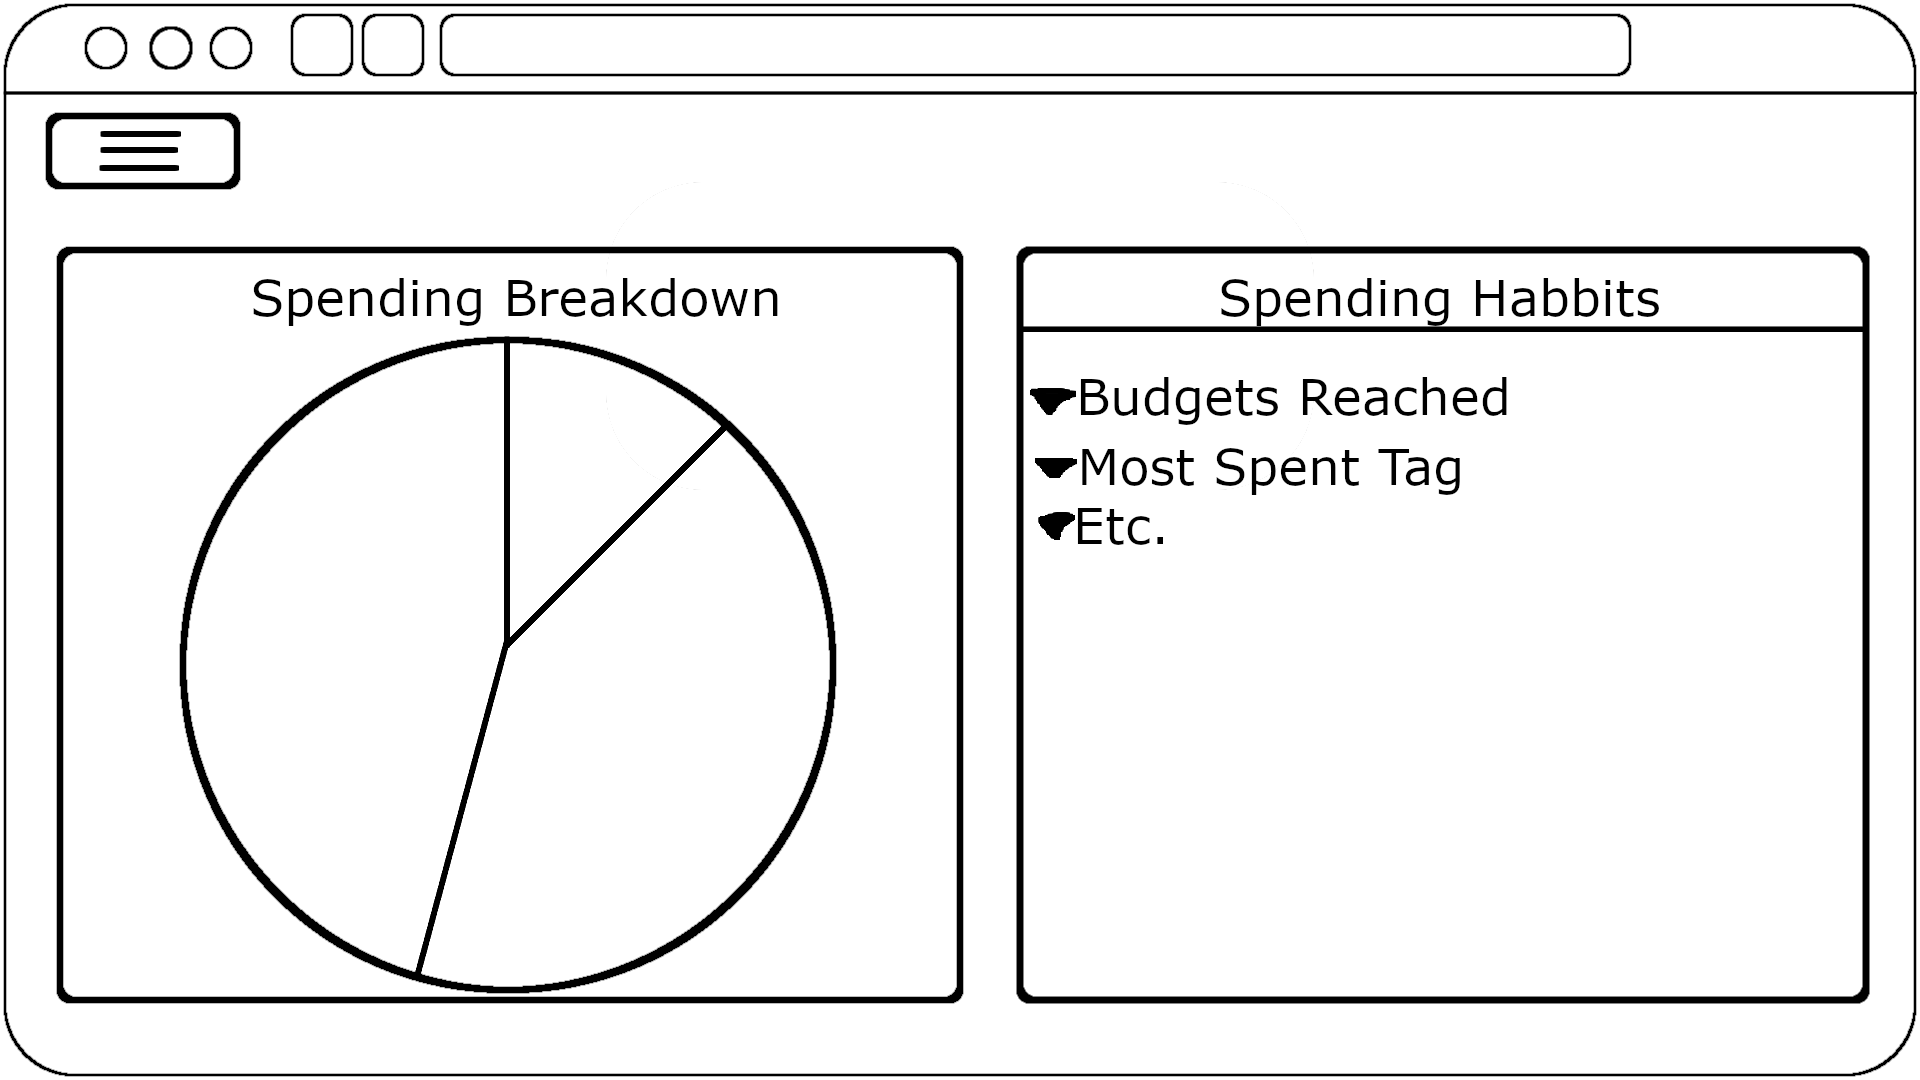
\includegraphics[width=3in]{StatsPage.png}\\
This page shows a breakdown of how much the user has been spending and shows the spending habits of the user. Note the dropdown menu up top, this is used to select what time period you'd like to look at, 1 month, 3 months, a year, or all time. The table below shows all transactions, and is default sorted by the name of the transaction, but you can click on the headings to either sort by those headings, or click a heading twice to switch to reverse sorting by that heading.\\
%==========================================================
\end{document}
%==========================================================